\documentclass[english,BCOR=4mm,cdfont=false]{tudscrreprt} % BCOR stellt die Bindekorrektur ein



% \documentclass[english,BCOR=4mm,cdfont=false]{tudscrreprt} %BCOR stellt die Bindekorrektur ein
% \KOMAoptions{parskip = half-}
% \iftutex
% \usepackage{fontspec}
% \else
% \usepackage[T1]{fontenc}
% \fi
% \usepackage{babel}
% \usepackage{isodate}
% \usepackage{isodate}
% \usepackage{svg}


% \usepackage{style} % all packages stored in here

% % --- TikZ und Zeichnungen ---
% \usepackage{tikz}
% \usetikzlibrary{
%   positioning,
%   calc,
%   shapes,
%   arrows.meta,  % Für moderne Pfeilspitzen (Latex, Stealth, etc.)
%   shapes.multipart,
%   fit           % Für group boxes
% }

% %\documentclass[11pt,a4paper]{article}
% %\usepackage[left=2.5cm, right=2.5cm, top=2.5cm, bottom=2.5cm]{geometry}
% \usepackage[onehalfspacing]{setspace}
% \usepackage{graphicx} % Required for inserting images
% \usepackage{pdfpages}
% %\usepackage[T1]{fontenc}


% \usepackage{amssymb,amsmath,amsthm, commath} % Diese Pakete sind nötig, um viele mathematische Formeln schreiben zu können.

% \usepackage[sorting = none]{biblatex} %Imports biblatex package
% \usepackage{csquotes}
% \addbibresource{idsysev.bib}
% %\bibliographystyle

% \usepackage{enumerate} % Ein Paket um individuelle Aufzählungen erzeugen zu können.

% \setlength\parindent{0em}

% \usepackage{blindtext}
% \usepackage{svg}

% PREAMBLE.TEX

% --- Core Setup ---

\usepackage[utf8]{inputenc} % Set input encoding to UTF-8 (standard)
\usepackage[T1]{fontenc}    % Use modern font encodings for PDF output
\usepackage[english, german]{babel}          % Proper hyphenation and language-specific settings
\usepackage{lmodern}        % Use the Latin Modern font
\usepackage{hyphsubst}      % Improved hyphenation

% --- Custom Style and Commands ---
% All visual styling, colors, and layout tweaks are in style.sty
\usepackage{style} 
\newcommand{\rarrow}{$\rightarrow$ }

%Mathematische Notation der gängigen Mengen
\newcommand{\RR}{\mathbb{R}} %reelle Zahlen
\newcommand{\CC}{\mathbb{C}} %komplexe Zahlen
\newcommand{\QQ}{\mathbb{Q}}
\newcommand{\NN}{\mathbb{N}}
\newcommand{\ZZ}{\mathbb{Z}}
\newcommand{\Prob}{\mathbb{P}} % Wahrscheinlichkeit

\newcommand{\gerquote}[1]{\glqq #1\grqq} %Deutsche Version der Anführungszeichen

% \newdateformat{myformat}{\THEDAY{ten }\monthnamengerman[\THEMONTH], \THEYEAR}

% --- Math Packages ---
\usepackage{amsmath}        % Advanced math environments
\usepackage{amssymb}        % Extra math symbols
\usepackage{mathtools}      % Further math tools, loads amsmath
\usepackage{commath}        % For common math commands like \dif
\usepackage{amsthm}         % For theorem and proof environments

% --- Tables and Figures ---
\usepackage{booktabs}       % For professional-quality tables
\usepackage{longtable}      % For tables that span multiple pages
\usepackage{tabulary}       % For tables with auto-adjusting column widths
\usepackage{tabularx}
\usepackage{graphicx}       % For including images
\usepackage{pdfpages}       % For including PDF pages
\usepackage{svg}            % For including SVG images
\usepackage{subcaption}     % For subfigures

% --- Document Utilities ---
\usepackage{listings}       % For code listings
\usepackage{csquotes}       % Context-sensitive quotation marks (required by biblatex)
\usepackage[sorting=none]{biblatex} % For bibliography management
\addbibresource{idsysev.bib}

% --- Referencing and Links ---
\usepackage{hyperref}
\hypersetup{
    colorlinks=true,
    linkcolor=tudblau,      % Defined in style.sty
    citecolor=tudblau,
    filecolor=tudrot,       % Defined in style.sty
    urlcolor=tudblau,
    pdftitle={Identification System Evaluation},
    pdfpagemode=FullScreen,
    linktoc=all             % Make links in ToC clickable
}
\begin{document}


\selectlanguage{german}
\faculty{Faculty of Electrical and Computer Engineering}
\institute{~ Institute of Communication Technology}
\chair{Deutsche Telekom Chair of Communication Networks}
\date{\today}
\title{Identification System Evaluation}
\subtitle{Hauptseminar Kommunikationssysteme \vspace{3cm}}
\subject{report}

\author{%
    Antonio Michael Hans Döring
    \matriculationnumber{}%
    \and%
    Armin Jacobi von Wangelin
    \matriculationnumber{}%
    \and%
    Nick Schubert
    \matriculationnumber{}
    \and%
    Caroline Weisser
    \matriculationnumber{}
}
\supervisor{M. Sc. Caspar v. Lengerke}
\maketitle

\newpage
\includepdf[pages = 4]{Alle Themen - HS KS SoSe2025.pdf}
\newpage


\chapter*{Selbständigkeitserklärung}
\thispagestyle{empty}
Wir versichern, dass wir die vorliegende Arbeit selbständig verfasst und keine 
anderen als die angegebenen Quellen und Hilfsmittel benutzt haben. Zur Verbesserung allein des sprachlichen Ausdrucks haben wir ChatGPT benutzt, ohne dass inhaltliche Änderungen vorgenommen wurden. Wir reichen sie erstmals als Prüfungsleistung ein. Uns ist bekannt, dass ein Betrugsversuch mit der 
Note \gerquote{nicht ausreichend} (5,0) geahndet wird und im Wiederholungsfall zum 
Ausschluss von der Erbringung weiterer Prüfungsleistungen führen kann.

\vspace{2cm}

% --- Improved Signature Layout ---
\noindent % Prevents indentation
\begin{minipage}[c]{0.45\textwidth}
    \vspace{4em} % Space for signature
    \hrule
    \centering
    Antonio Michael Hans Döring
\end{minipage}
\hfill
\begin{minipage}[c]{0.45\textwidth}
    \includegraphics[height=4em]{images/Armin Unterschrift.png}
    \hrule
    \centering
    Armin Jacobi von Wangelin
\end{minipage}

\vspace{3cm}

\noindent % Prevents indentation
\begin{minipage}[c]{0.45\textwidth}
    \includegraphics[height=4em]{images/unterschrift_nick.png}
    \hrule
    \centering
    Nick Schubert
\end{minipage}
\hfill
\begin{minipage}[c]{0.45\textwidth}
    \includegraphics[height=4em]{images/Caro_Unterschrift-1.png}
    \hrule
    \centering
    Caroline Weisser
\end{minipage}

\vspace{3cm}
\noindent Dresden, den 25.07.2025

\newpage
\selectlanguage{english}
\begin{abstract}
    \begin{center}
        \textbf{Abstract}
    \end{center}
This report presents a systematic evaluation of noiseless identification (ID) systems with a focus on ID tagging codes, extending the framework of goal-oriented communication beyond traditional Shannon-theoretic limits. ID codes are designed to enable the transmission of reduced information, thereby decreasing bandwidth consumption. The receiver verifies the occurrence of a specific event rather than deducing information out of the message. A modular Python-based test framework is developed to analyze various ID coding schemes, including Reed-Solomon, Reed-Muller, and cryptographic hash-based encoders, across a wide range of parameters. The framework is designed to support large-scale parameter sweeps, ensure reproducible experiments, and provide interactive visualization of key metrics such as false positive ratio, execution time, code rate, and Hamming distance statistics. The simulations confirm existing findings for false positive probabilities.

Additional scenarios, including k-Identification and multiple tag transmissions, are investigated to assess their impact on system reliability and computational overhead. It is derived and demonstrated by simulation that multi-tag strategies exponentially reduce collision probability at the cost of a linear decrease in code rate. To address this problem, a protocol of subsequent tag transmission is introduced.\\
Furthermore, the behavior of ID codes under non-random message distributions is analyzed, revealing that certain encoders, particularly Reed-Solomon and cryptographic hash-based schemes, effectively randomize structured inputs, whereas Reed-Muller codes exhibit notable weaknesses in these cases.

Fundamental trade-offs between reliability, computational complexity, and code rate in the design of practical ID systems are highlighted. By combining empirical findings with theoretical bounds, the report provides deeper insights into the optimization of ID coding schemes for applications in resource-constrained and event-driven communication systems, such as Industry 4.0, IoT networks, and digital twin synchronization.

\newpage
\selectlanguage{german}
    \begin{center}
        \textbf{Kurzfassung}
    \end{center}
Dieser Bericht stellt eine systematische Evaluation von rauschfreien Identification-Systemen (ID Systems) mit Schwerpunkt auf ID Tagging Codes vor, wodurch der Rahmen zielorientierter Kommunikation über die klassischen Grenzen der Shannon-Theorie hinaus erweitert wird. ID Codes ermöglichen die Übertragung einer reduzierten Menge an Information und senken so den Bandbreitenbedarf. Der Empfänger verifiziert das Eintreten spezifischer Ereignisse, anstatt Information aus der Nachricht zu extrahieren. Ein modular aufgebautes, Python-basiertes Testframework wurde entwickelt, um verschiedene Codierungsschemata, darunter Reed-Solomon-, Reed-Muller- und kryptografische Hash-basierte Verfahren, über einen weiten Parameterbereich hinweg zu analysieren. Das Framework unterstützt groß angelegte Parameter-Sweeps, gewährleistet Reproduzierbarkeit und ermöglicht interaktive Visualisierungen zentraler Metriken wie False Positive Ratio, Ausführungszeit und Coderate.

Weiterführende Szenarien, wie k-Identification und das Übermitteln mehrerer Tags, werden hinsichtlich ihres Einflusses auf die Systemzuverlässigkeit und den Rechenaufwand untersucht. Dabei wird theoretisch und simulativ demonstriert, dass Multi-Tag-Strategien die Kollisionswahrscheinlichkeit exponentiell reduzieren, jedoch die Coderate linear senken. Um dieses Problem zu beheben wird ein Protokoll der nacheinanderfolgenden Übermittlung von Tags vorgestellt. \\
Darüber hinaus wird das Verhalten von ID Codes bei deterministischer Verteilung der Nachrichten untersucht.  Dabei zeigt sich, dass insbesondere Reed-Solomon- und kryptografische Hash-Verfahren strukturierte Eingaben effektiv randomisieren, während Reed-Muller-Codes in diesen Fällen deutliche Schwächen aufweisen.

Grundlegende Kompromisse zwischen Zuverlässigkeit, Rechenkomplexität und Coderate beim Entwurf praktischer ID-Systeme werden herausgearbeitet. Durch die Kombination empirischer Ergebnisse mit theoretischen Grenzen gibt der Bericht tiefere Einblicke in die Optimierung von ID Codes für Anwendungen in ressourcenbeschränkten und ereignisgetriebenen Kommunikationssystemen, wie etwa Industrie 4.0, IoT-Netzwerken und der Synchronisation digitaler Zwillinge.
\end{abstract}
\selectlanguage{english}
\tableofcontents

\newpage

\chapter*{List of Symbols and Abbreviations}

\begin{longtable}{@{}p{0.2\textwidth} p{0.75\textwidth}@{}}
\toprule
\textbf{Symbol} & \textbf{Description} \\
\midrule
\endfirsthead
\toprule
\textbf{Symbol} & \textbf{Description} \\
\midrule
\endhead
\bottomrule
\endfoot
\bottomrule
\endlastfoot

% --- General Parameters ---
\multicolumn{2}{l}{\textbf{General Parameters}} \\ \addlinespace
$\boldsymbol{a}, \boldsymbol{b}$ & Message vectors at the sender and receiver, respectively. \\
$\boldsymbol{m}, \boldsymbol{u}$ & General notation for a message vector, often used as input to an encoder. \\
$\mathbf{c}$                 & Codeword vector produced by a Forward Error Correction (FEC) encoder. \\
$N$                          & Total number of messages in the message space. \\
$\tilde{N}$                  & Effective number of messages in a reduced ID problem after grouping messages. \\
$n_\text{ID}$                & Message ID length in bits, representing a specific message index. Often calculated as $n_\text{ID} = \lceil \log_2(N) \rceil$. \\
$n_\text{cue}$               & Size in bits of the transmitted cue, which consists of the tag(s) and possibly their respective position. \\
$t, t_a$                     & A single tag; $t_a$ specifically denotes the tag generated from message $\boldsymbol{a}$. \\
$q$                          & Tag symbol alphabet size, often equivalent to the order of the Galois Field. \\
$\mathbb{F}_q$               & The Galois Field containing $q$ elements. \\
$T, T_\text{max}$           & Number of tags transmitted in Multi-Tag systems. $T_\text{max}$ is the maximum number of tags in a sequential transmission protocol. \\
$k$ (in k-ID)               & The number of distinct messages in the set $B$ for a k-Identification scenario. \\
$B$                          & A set containing $k$ distinct messages, defined as $B = \{\boldsymbol{b_1}, \dots, \boldsymbol{b_k}\}$. \\
$W$                          & The Hamming weight (number of non-zero symbols) of a codeword, relevant for Constant-Weight Codes (CWC). \\
$K$                          & The maximum overlap between two codewords, i.e., the greatest number of identical symbols at identical positions. \\
$G$                          & The generator matrix of a linear block code. \\
$\pi$                        & The fixed position (index) of the codeword from which a tag is extracted. \\
\midrule

% --- Performance Metrics ---
\multicolumn{2}{l}{\textbf{ID Metrics}} \\ \addlinespace
$R$                       & The single-tag ID code rate, defined as $R = \log(n_\text{ID}) / n_\text{cue}$. \\
$R_T$                     & The effective ID code rate when transmitting $T$ tags simultaneously. \\
$r$                       & Overall system reliability, denoting the fraction of correct identification results. \\
$\overline{p_\text{fp}}$  & Empirically measured mean False Positive (FP) ratio; the ratio of FP events to all true negative cases. \\
$p_\text{fp, k}$      & The mean FP probability in a k-ID scenario with a set of size k. \\
$p_\text{fp, T}$            & The mean FP probability when using $T$ tags for verification. \\
$\lambda_2$, $\lambda_{fp}$ & The theoretical upper bound on the FP probability for a single tag. \\
$\lambda_{fp}^{(T)}$            & The theoretical upper bound on the FP probability when using $T$ tags.  \\
\midrule

% --- Probabilistic & Entropy Concepts ---
\multicolumn{2}{l}{\textbf{Probability and Information Theory}} \\ \addlinespace
$\mathbb{P}(\cdot)$       & The probability of an event. \\
$p_c$                     & The theoretical tag collision probability\\
$p_{tp}$                  & True Positive Ratio: the a priori probability that sender and receiver messages are identical, i.e., $\mathbb{P}(\boldsymbol{a}=\boldsymbol{b})$. \\
$p_M(\cdot), p_T(\cdot)$ & Probability Mass Functions (PMF) over the message and tag alphabets, respectively. \\
$H_2(p)$                   & The Rényi entropy of order 2, also known as the collision entropy, for a distribution $p$. \\
$G_2$                     & The normalized Rényi-2 entropy gain metric, measuring the effectiveness of an encoder in creating a uniform tag distribution. \\
$D_2(P \| Q)$             & The Rényi divergence of the second order between two probability distributions $P$ and $Q$. \\
$\hat{v}, \hat{v}_\text{fp}$ & The equality estimate at the receiver: $\hat{v}_\text{fp}$ indicates a false positive. \\
\midrule

% --- Code-Specific Parameters ---
\multicolumn{2}{l}{\textbf{Code-Specific Parameters}} \\ \addlinespace
\textbf{Reed-Solomon} &  \\
$k$                         & The dimension of an RS code (number of message symbols). \\
$k_o$                       & The dimension of the outer RS code in a concatenated (RS2) scheme. \\
$k_i$                       & The dimension of the inner RS code in a concatenated (RS2) scheme. \\
$n_i$                      & The symbolic length of the inner Reed-Solomon codewords. \\
\addlinespace
\textbf{Reed-Muller}   &  \\
$m$                         & The generation parameter of an RM code, related to the number of variables. \\
$r$                         & The order (degree) parameter of an RM code. \\
\end{longtable}

\chapter{Introduction}

\section{ID Codes}
\label{sec:idCode}
To meet the rapidly growing demand for data transmission, approaches beyond conventional lossless compression have become essential.
The ongoing digitalization of society has resulted in unprecedented growth in global data traffic, which has maintained an average annual increase of more than 20\% in recent years~\cite{cisco2023annual}. High-definition and ultra-high-definition video streaming already accounts for over 70\% of all IP traffic and is expected to exceed 80\% in the near future~\cite{cisco2018vni}. Popular social media platforms such as Instagram, TikTok, and YouTube amplify this trend through short-form, high-resolution videos and live interactive content, which require substantial throughput and low latency. Simultaneously, the digital transformation of work, driven by remote collaboration, the proliferation of IoT devices, and AI-based cloud services further intensifies bandwidth requirements, with billions of connected devices generating continuous data streams~\cite{edgeoptic2024traffic}.
While traditional lossless compression techniques remain effective within their theoretical limits, they cannot alone accommodate the exponential rise in data exchange. As ultra-high-resolution video, immersive AR/VR experiences, and massive-scale data synchronization become increasingly commonplace, communication networks face growing strain, necessitating novel strategies for scalable and efficient data transmission.

Pushing the boundaries set by Claude Shannon’s source coding theorem \cite{The_mathematical_theory_of_communication} to the limits and beyond, Post-Shannon theory finds ways to extend classical information theory, with a focus on goal-oriented and resource-aware communication \cite{strinati2021beyondShannon}. In the context of goal-orientation, one approach is to shift the focus from the technical to the semantic problem by specifying a communication goal apart from a transmission of the whole message. 
If the specific communication goal differs from reproducing the sender's message at the receiver, codes can compress data below the previous theoretical limit. In this report, that is part of the \textit{Hauptseminar Kommunikationssysteme} at TU Dresden, we will set our focus on the identification (ID) problem, where a receiver aims to verify whether a received message matches its own message. 
Namely, both the sender and the receiver are aware of a common finite set of possible messages. The sender does not transmit the whole message but selects one out of this set and transmits a representation of this message (ID message) being shorter than the original. The receiver similarly chooses a message and compares the corresponding ID message to the received one. If it may determine whether they are the same (in other words if they are identical), the communication goal is interpreted as fulfilled \cite{Codes_for_ID_Tutorial}. Equality then is a one bit property: it can either be true or false. \\
Addressing the ID problem using full message transmission presents a valid solution, nevertheless using goal-oriented ID codes enables achieving the identification goal much more efficiently than using general-purpose channel codes.

To summarize, ID encoding reduces the information content of a message. It thereby introduces a non-zero error probability, which needs to be small enough to reliably achieve the specific communication goal of identification. In some cases, e.g. with linear block encoding, this error probability can be bounded to an upper limit. \\
The collision probability is the price for ID codes that support up to exponentially more messages under the same conditions than standard message transmission. 
Putting it into other words emphasizes the relevant trade-off: the smaller the collision probability bound, the larger the codeword has to be. It is a current task to find ways to overcome known limitations by various techniques like sending multiple tags (see also section \ref{sec:multiple-tag transmission}), smaller symbol sizes or extending known codes \cite{deppe_ferrara_2020}. These approaches try pushing towards the optimum in the top left corner of figure \ref{fig:qualiPlot}. From a practical viewpoint, larger codewords come at the cost of processing overhead. The designer's task then is to adjust the ID system to application specific needs, for instance a minimal error bound for safety relevant applications or a slightly higher bound for IOT. 

ID codes may find application in protocols including radio frequency identification systems, digital twins and synchronization \cite{ID_Codes_Topical_Review}.
"[Sensors] first apply a binary hypothesis test to decide whether they are the targeted sensor. If this is not the case, they do not decode the command" \cite{ibrahim2021idcodes}. In this case, a wrong identification comes at the cost of wasting power, yet nobody gets harmed. Some wrong identification might be acceptable, if processing power is being saved.

\begin{figure}[h!]
    \centering
    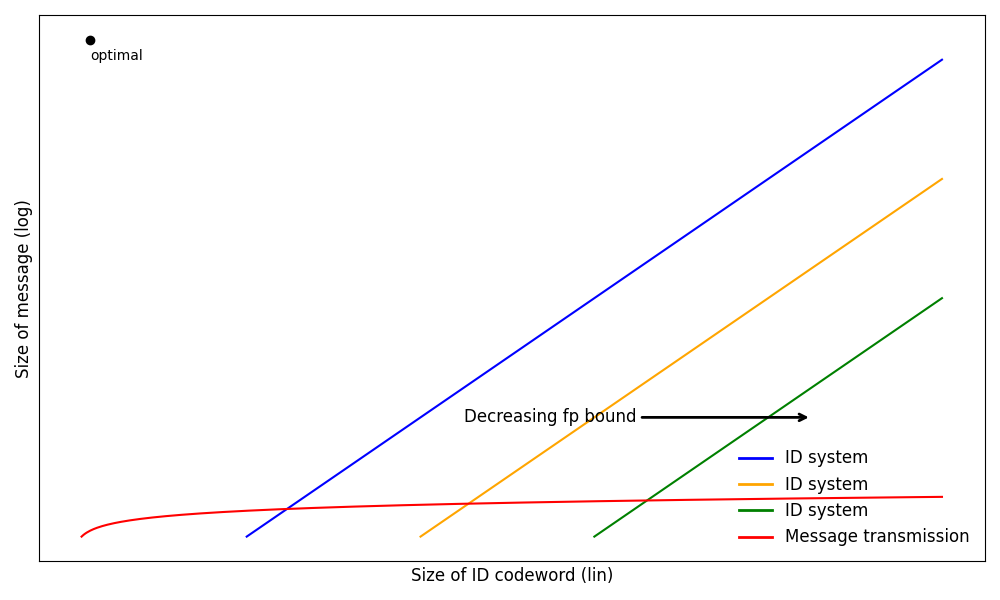
\includegraphics[width=0.8\linewidth]{images/qualitative_figure.png}
    \caption{Qualitative comparison of ID systems of different error probability bounds to message transmission.}
    \label{fig:qualiPlot}
\end{figure}

In this report, we examine the performance of a specific class of ID codes known as noiseless ID tagging codes. We evaluate the influence of various code parameters on key performance metrics such as error probability, execution time, and code rate. To facilitate this analysis, we developed a test framework and an interactive dashboard to visualize the results. Beyond verifying existing findings, we extend the evaluation to several modified scenarios, including k-Identification, the use of multiple tags, and the impact of non-random message patterns. This report aims to provide a deeper, more intuitive understanding of the trade-offs involved in designing practical ID systems.

\section{Distribution of Tasks}
To ensure an efficient workflow, the task was divided among the four team members. Nick was primarily responsible for implementing the Python framework described in \ref{sec:testFramework} and provided example scripts for metric analysis to facilitate replication by the others. Throughout the course of the project, he modified various parts of the code as our ideas evolved---particularly following discussions with our supervisor Caspar, which led to adjustments in the project's direction. Also, he is responsible for the analyses concerning non-random message patterns and provided feedback to the \texttt{idcodes} library's developers for performance and documentation updates.

Since the \texttt{idcodes} library was initially not publicly available, a shared development platform was required. Armin addressed this problem by setting up a Docker container running an Ubuntu 24.04 system, where the prototype of the \texttt{idcodes} library was run. He came up with a test framework architecture allowing all team members to conduct simulations independently in order to identify metrics of potential interest for further analysis. Later on, he also implemented the functionality to gather all of the interesting data in a structured way. This includes periodic saving of results, resume capability from previous checkpoints, progress tracking using metadata as well as automatic backup creation. This enabled processing the huge amounts of data needed to support the theoretical findings, without the risk of losing any data points.

To determine which metrics to focus on, we held a brainstorming session to explore possible directions. Each team member then selected a topic they found promising. Caroline reviewed the suggested literature to us to build a theoretical foundation for understanding identification systems. This background was essential for evaluating the framework's correctness and for assessing whether the calculated metrics were meaningful in the intended context. It also gave us a better idea on which simulations would give interesting results or end in obvious proofs of the basic theory. Furthermore, she expanded the theory to the k-Identification and multiple tags scenario, challenging the gains, opportunities and limits of these modifications of the ID problem.

Antonio contributed to the analysis as well as idea gathering for the metric evaluation. After the direction of the project was set, he researched various design approaches for presenting the results. They should be shown in the form of graphs and numerical indicators within a dashboard. He then implemented this dashboard with a focus on clarity, usability, and visual appeal.

The written part of the report was structured as follows, with responsibilities divided among the team members:\\
Antonio authored the description of the dashboard in \ref{sec:metVis} as well as the evaluation and interpretation of the results in \ref{chap:evalInter}.\\
Armin first gave a general introduction into ID Codes in \ref{sec:idCode}, put down the test framework architecture in \ref{sec:testFramework} and then shifted the view to future task by giving an outlook in \ref{sec:outlook}.\\
Caroline was responsible for the description of ID systems in \ref{sec:backgroundIdCodes} and \ref{sec:perfId}, as well as the introduction of advanced scenarios in \ref{sec:VerIdprob} and theoretical examinations of k-Identification and multiple tags in \ref{sec:kIdent} and \ref{sec:multTag}. She presented the results and discussion of these in the theoretical part of \ref{sec:FindingskID}.\\
Nick wrote the sections on the methods used in the framework (\ref{sec:metrics_methods}), System Reliability and False Positive Ratio (\ref{sec:sysRel}) and Analysis with Non-Random Message Patterns (\ref{sec:collision_prob}, \ref{sec:nonRandom}, and \ref{sec:mesPat}), as well as the summary (\ref{sec:summary}).\\
The abstract and Kurzfassung were written by Armin and Caroline in cooperation.


\chapter{Background}

\section{Noiseless ID Tagging Codes}
\label{sec:backgroundIdCodes}
ID tagging codes are a class of ID codes which rely on the transmission of a single tag. A tag is a single symbol of the error-correction codeword at a fixed (possibly randomized) position. This allows a double-exponential scaling of the message length and hence the number of possible messages at the same code rate. The cost is an inherent positive error probability due to the fact that the symbol space is smaller than the message space. As a result, several messages can lead to the same tag (\cite{Codes_for_ID_Tutorial}, Sections III, VI, VII). 
The encoding process comprises the coding of the message into an forward error correction (FEC) codeword. This is a repurpose of FEC codes for the advantage of larger Hamming distances and thus a lower tag collision probability, which comes at the cost of a message size increase.
The FEC codeword can be obtained by different linear block coding schemes, like Reed-Solomon (RS1), concatenated Reed-Solomon (RS2) or Reed-Muller (RM) \cite{ID_Codes_Topical_Review}. 
Afterwards, one symbol in the FEC codeword (the tag) is transmitted. In case the receiver does not know the position, it has to be transmitted additionally (\cite{Codes_for_ID_Tutorial}, Section VII.A).

In this report, we examine the performance of noiseless ID tagging codes. Namely, we assume an error-free transmission of a tag. The encoding process is deterministic and the tag position is known to the receiver. Hence, two distinct tags never stem from the same message. For this reason, no false negative errors may occur. This is explained in \cite{ID_Codes_Topical_Review}, Section II.B and \cite{Codes_for_ID_Tutorial}, Section VI.C  as well: 

\begin{quote}
"Noiseless-ID codes are subject to FP errors but not to FN
errors. That is because each message $\boldsymbol{u}$ is associated with a
 single noiseless-ID codeword subset $\mathcal{C}_u$ for both the encoding
 and verification step. If the message pair $(\boldsymbol{a}, \boldsymbol{b})$ matches, i.e.,
 $\boldsymbol{a} = \boldsymbol{b}$, then the equality estimate $\hat{v}$ is always correct and
 no FN errors occur. For message pairs $(\boldsymbol{a}, \boldsymbol{b})$ of differing
 messages $\boldsymbol{a} \neq \boldsymbol{b}$, the ”hashing” of the message $\boldsymbol{a}$ can result
 in FP errors $\hat{v}_{\text{fp}}$ because the codeword subsets $\mathcal{C}_u$ overlap."
\end{quote}

A notable advantage of the FEC codes are their capability to guarantee an upper bound for false-positive errors. The concrete bound depends on the type and the internal parameters of the code and are presented in the following section.

\section{Performance of CWC-based ID Codes}
\label{sec:perfId}
In \cite{ID_Codes_Topical_Review}, performance metrics of different linear block codes with constant-weight initialization (CWC) have been examined. CWC are characterized by each symbol having the same hamming weight (number of bits not equal to 0). In the article, RM, RS1 and RS2 codes have been used as linear block codes and each symbol is then coded in CWC. Mostly, PPM initialization is used, where the symbols represent a one-hot encoding. The metrics include the mean error probability, the error probability bound for order 2 errors (since only false positive errors may occur) and the code rate. An ID code rate is introduced to clarify the double exponential scaling of ID codes, defined as 
\begin{equation}
    R = \frac{\log(\log(N))}{n_\text{cue}} = \frac{\log(n_\text{ID})}{n_\text{cue}}
\end{equation} with N being the number of messages and $n_\text{cue}$ the cue size (\cite{ID_Codes_Topical_Review}, eq. 16). A cue comprises the tag and its size therefore depends on the tag symbol size. The existence of an error probability bound is a decisive advantage of the used block codes compared to hash-functions. This is considered crucial for use cases with very high reliability requirements.

Briefly, the CWC initializations appear to have little influence and the performances differ rather between the linear block codes. The authors examined the influence of the tag symbol size $q$ as well as the generation $m$, order $r$ and dimensions $k, k_i, k_o$ of RM and RS, respectively, for a fixed number of messages $2^{n_\text{ID}}$. Here, $q$ is equivalent to $n_\text{cue}$ since a tag is one symbol.
For every block code, a large tag symbol size achieves the lowest error metrics and should therefore be chosen as large as possible with reasonable computational effort. It determines the mean error probability for all block codes as 
\begin{equation}
    p_\text{fp} = \frac{1}{q},
\end{equation} 
while the notation for this quantity is $\overline{p_{err}}$.\\
For RS2 codes, the outer Reed-Solomon code's dimension $k_o$ should be chosen as high as possible, while the inner RS dimension $k_i$ should be kept low, provided the constraint $k_0 \leq q^{k_i - 1}$ is satisfied. For Reed-Muller codes, the parameter $m$ should be set as high and $r$ as low as possible, within the constraint $m \leq r$.

Regarding the error probability bound $\lambda_2$, the general expression is (\cite{ID_Codes_Topical_Review}, eq. 17)
\begin{equation}
    \lambda_2 = \frac{K}{W}, 
\end{equation}
where $K$ is the maximum overlap between two codewords (number of the symbols two codewords share in the worst case) and $W$ the hamming weight. Both are properties of the FEC codes in combination with the respective CWC initialization, summarized in \cite{ID_Codes_Topical_Review}, table 2. The most relevant are:
\begin{itemize}
    \item PPM-RS1: $\lambda_2 = \frac{k-1}{q-1}$
    \item PPM-RS2: $\lambda_2 = \frac{k_o - 1}{q^{k_i}} + \frac{(k_i - 1)(q^{k_i} - k_o)}{(q-1)(q^{k_i} - 1)}$
    \item PPM-RM: $\lambda_2 = \frac{r}{q}$
\end{itemize}

\section{Advanced ID Scenarios}
\label{sec:VerIdprob}
\subsection{k-Identification}
A modification of the ID problem is the k-Identification (k-ID) problem (as introduced in \cite{Codes_for_ID_Tutorial}, Section X.B as $K$-ID). In this scenario, the receiver does not need to know whether the messages are perfectly identical. It is rather sufficient to gain information within a certain tolerance. 
Therefore, the receiver wants to determine whether the message $\boldsymbol{a}$ is identical to at least one message of a set of k messages $B = \{\boldsymbol{b_1},...,\boldsymbol{b_k}\}$, namely if 
$\boldsymbol{a} \in B$. Hence, the verification is positive if the tag of $\boldsymbol{a}$ matches one of the tags in $B$: $t_a \in \{t_{b_1},...,t_{b_k}\} = t_B$.

\subsection{Multiple-Tag Transmission}
\label{sec:multiple-tag transmission}
To improve the reliability of an Identification system, one may consider increasing the number $T$ of sent tags (proposed in \cite{Codes_for_ID_Tutorial}, Section VII.D). As a consequence, both the false positive ratio and the ID code rate are expected to diminish. \\
With $n_i$ being the number of dimensions of the Galois Field in the inner RS code, the choice of multiple tag becomes non-trivial. For \texttt{RS2ID} systems, positions of multiple tags  should differ in at least $n_i$ symbols due to the structure of concatenated Reed-Solomon-Codes \cite{von_lengerke_identification_2023}: 
\begin{quote}
    "Instead of sending multiple adjacent tags, tags from different
    inner RS codewords should be transmitted. For that reason, the
    deterministic distance between the positions of multiple tags
    should be at least the length $n_i$ of an inner RS codeword." 
\end{quote}

\section{Collision Probability and Optimal Tag Distribution} 
\label{sec:collision_prob}
As will become evident in the system reliability discussion (section \ref{sec:sysRel}), a critical performance indicator for the ID system is the false positive ratio. For clarity, we distinguish between the empirically estimated mean false positive ratio, $\overline{p_\text{fp}}$ and its theoretical foundation, the tag collision probability $p_c$. The collision probability is the likelihood that two tags, drawn independently from a tag distribution $p_T(t)$, are identical. 
Let $M$ be a random vector of length $k$ representing a message, with symbols drawn from an alphabet $\mathcal{M}$. The corresponding tag, a random variable $T$, is drawn from an alphabet $\mathcal{T}$. For this analysis, we operate in the Galois Field $\mathbb{F}_{256}$, so the alphabets are composed of $q=256$ symbols, and $\mathcal{M}, \mathcal{T} \subseteq \mathbb{F}_{256}$.
For a discrete distribution, the tag collision probability $p_c$ is calculated by summing the squared probabilities of each outcome:
\begin{equation}
p_c = \sum_{t \in T} p_T^2(t)
\end{equation}
This is a generalization of the classic birthday problem to non-uniform distributions \cite{feller1968introduction}. To minimize false positives, an ideal encoder should produce a tag distribution that minimizes this collision probability.

We can derive the optimal distribution that minimizes $p_c$ using the Cauchy-Schwarz Inequality (CSI) \cite{steele2004cauchy}. For any two vectors $\vec{a}, \vec{b} \in \mathbb{R}^n$, the inequality states:
\begin{equation}
\left(\sum_{i=1}^n a_i b_i\right)^2 \leq \left(\sum_{i=1}^n a_i^2\right) \left(\sum_{i=1}^n b_i^2\right) \label{eq:CSI}
\end{equation}
Equality holds if and only if $\vec{a}$ and $\vec{b}$ are linearly dependent \cite{steele2004cauchy}. Let the tag alphabet size be $|\mathcal{T}| = q$. We define our vectors as:
\begin{align*}
    \vec{a} &= (p_T(t_1), p_T(t_2), ..., p_T(t_q)) \\
    \vec{b} &= (1, 1, ..., 1)
\end{align*}
Substituting these into the CSI \eqref{eq:CSI} yields:
\begin{align*}
    \left(\sum_{i=1}^q p_T(t_i) \cdot 1\right)^2 &\leq \left(\sum_{i=1}^q p_T(t_i)^2\right) \left(\sum_{i=1}^q 1^2\right) \\
    \left(1\right)^2 &\leq (p_c) \cdot (q)
\end{align*}
This provides the theoretical lower bound for the collision probability:
\begin{equation}
    p_c \geq \frac{1}{q}
\end{equation}
The minimum collision probability is achieved when the equality in the CSI holds, which occurs when $\vec{a}$ and $\vec{b}$ are linearly dependent. This implies $p_T(t_i) = k$, $i = 1,2,...,q$ for some constant $k$. As the probabilities must sum to one, $\sum_{i=1}^q k = qk = 1$, so $k = 1/q$. The uniform distribution is optimal, minimizing the collision probability to $p_c = 1/q$ \cite{cover2006elements}. An effective encoder should therefore transform any input message distribution into a tag distribution that is as close to uniform as possible.


\chapter{Methodology}

We evaluate the influence of the code parameters on different performance metrics of ID systems, such as the mean and worst case error probability, execution time and code rate. 
Finding an optimum between these metrics, mutually effecting each other, often depends on the specific use case of the identification system. This includes the physical or semantic interpretation of each message, the constraints the system is underlying and the role it takes in a larger communication protocol. \\
Within our report, we developed a test framework, simplifying the process of finding suitable code parameters by visualizing code metrics data in an intuitive dashboard. 
The simulation results are produced using the python library \texttt{ecidcodes} (initially \texttt{idcodes}) \cite{ecidcodesLib}. The changeable parameters are the message generation, message length, tag position and size of the Galois Field the codes operate in. To eliminate one degree of freedom, the tag position remains fixed. 

\section{Analysis of System Reliability}
\label{sec:sysRel}
For a real-life applicable ID system, it is crucial to look at its reliability $r$. Suppose the sender has message $\mathbf{a}$ and the receiver message $\mathbf{b}$. Naively, the following definition comes to mind:
\begin{equation}
    r \coloneq \frac{c}{N},
\end{equation}
where $c$ is the number of correct identification results, i.e. a correct positive estimate in case both sender and receiver have the same message $(\mathbf{a} = \mathbf{b})$, and a correct negative estimate provided different messages $(\mathbf{a} \neq \mathbf{b})$. $N$ refers to the total number of messages processed by the identification system. \\
In a real system, the equality of $\mathbf{a}$ and $\mathbf{b}$ might appear with varying likelihood. We define the true positive ratio $p_\text{tp}$ as the probability that sender and receiver share the same message, in other words:
\begin{equation}
    p_\text{tp} \coloneq \mathbb{P}(\boldsymbol{a} = \boldsymbol{b}). 
\end{equation}

\begin{figure}[h!]
    \centering
    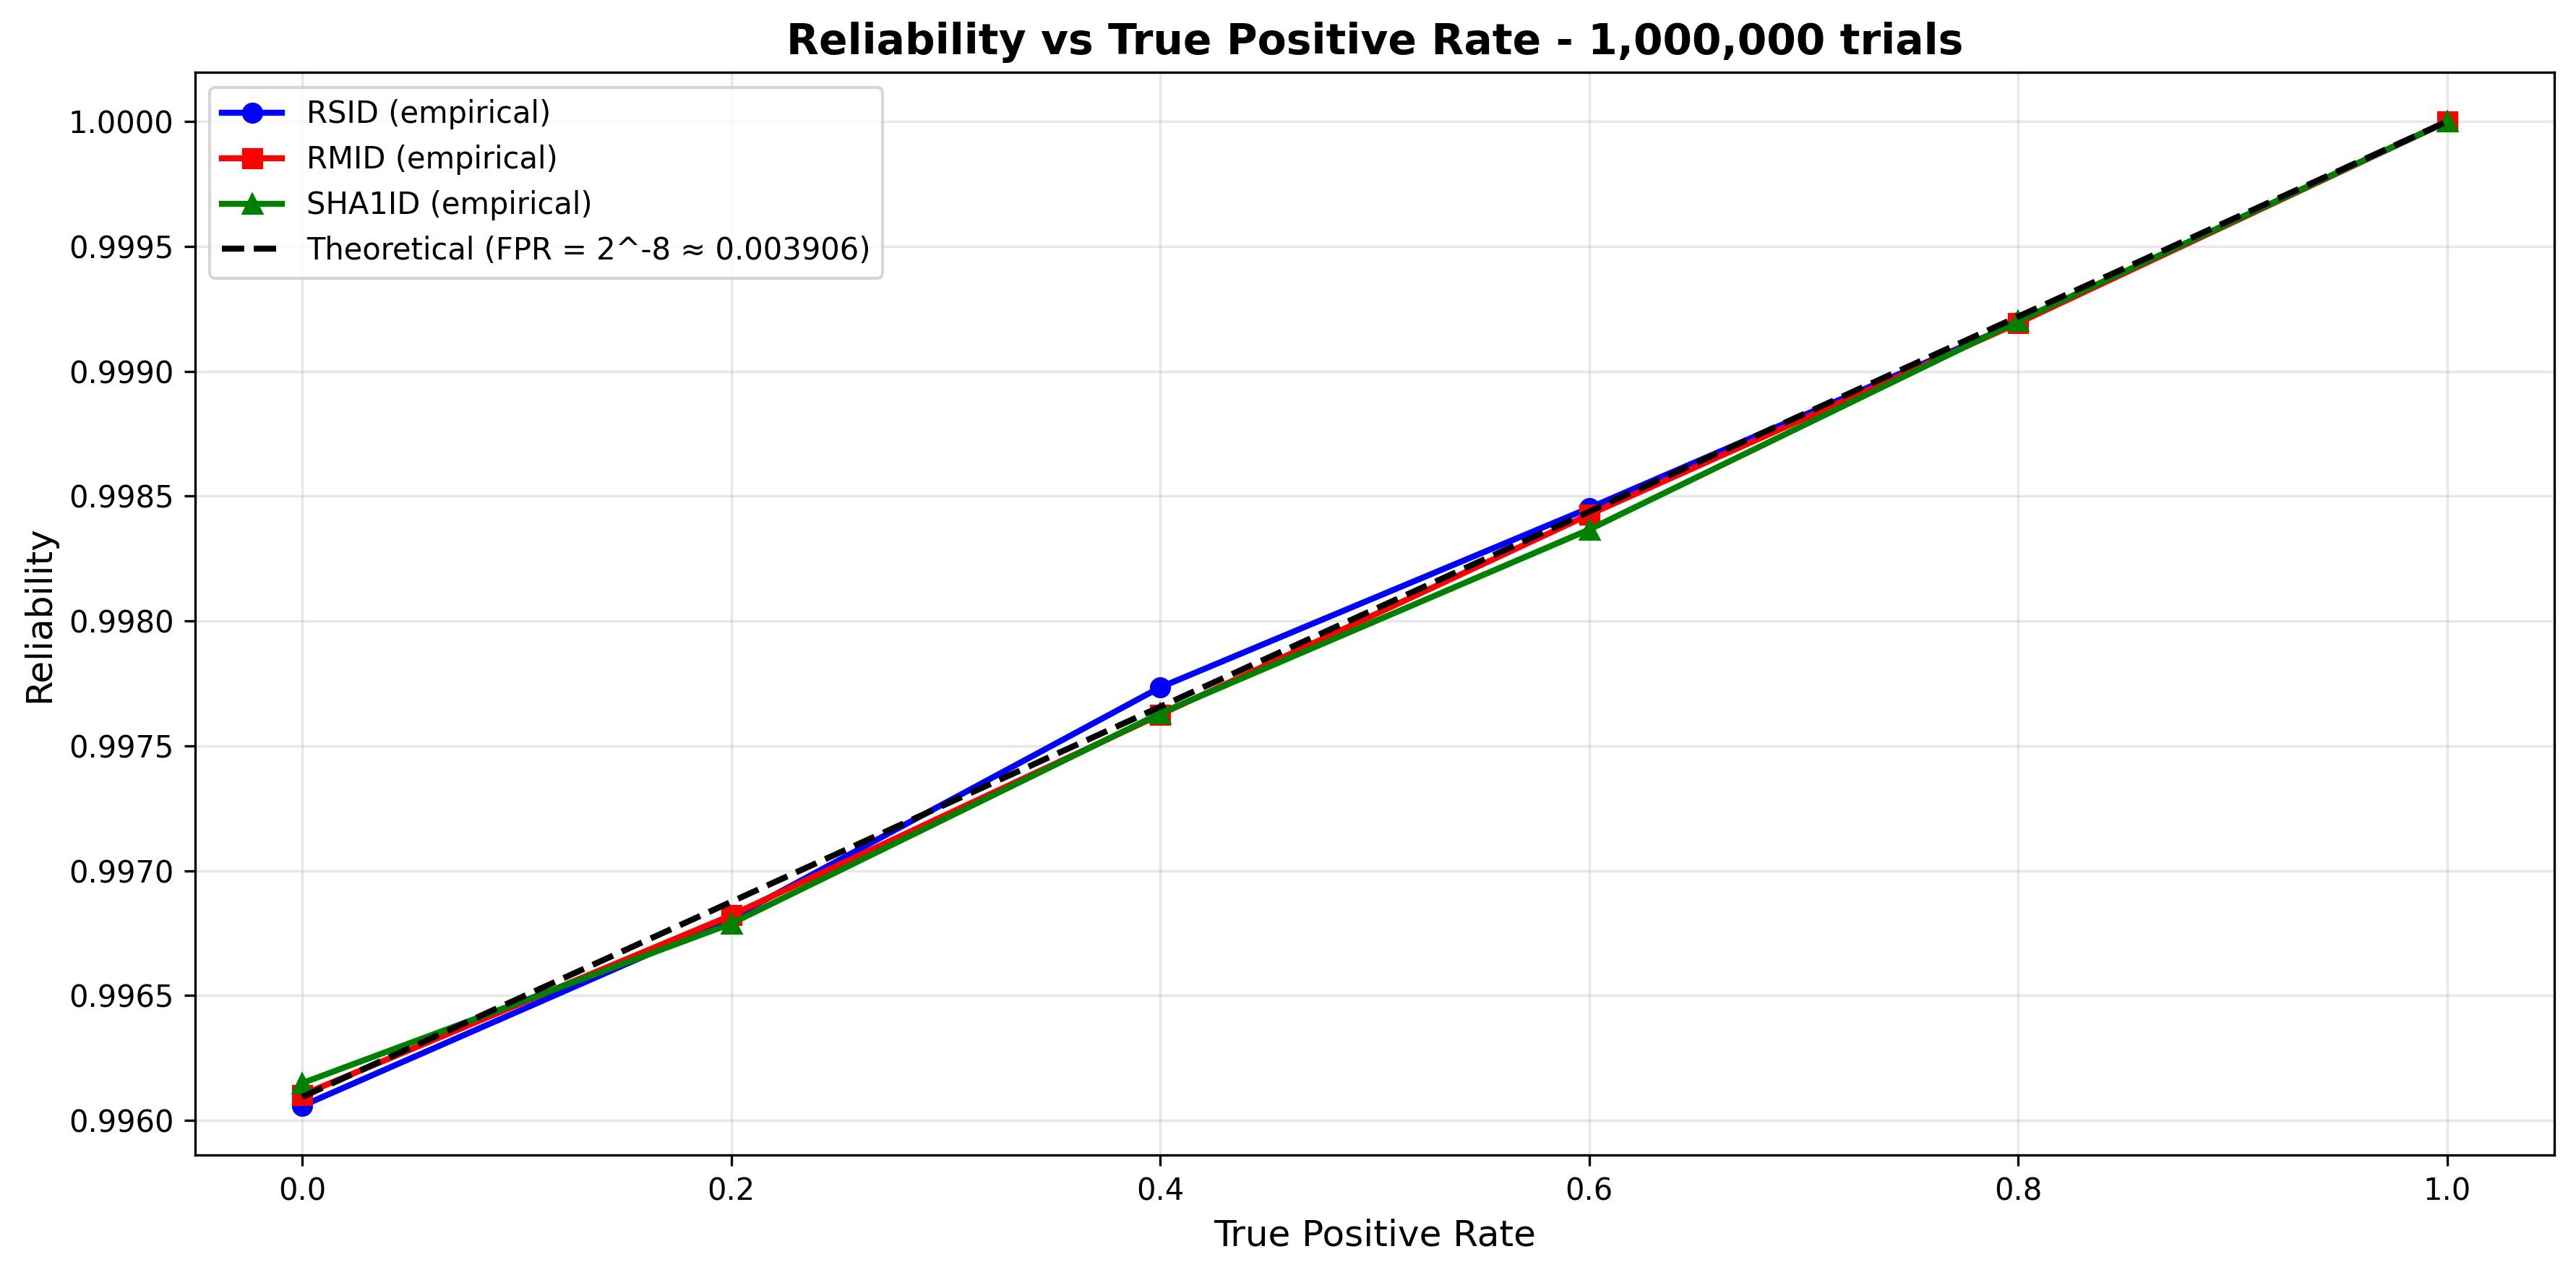
\includegraphics[width=0.75\linewidth]{plots/reliability_comparison.png}
    \caption{$r$ vs. $p_\text{tp}$ for \texttt{RSID}, \texttt{RMID} and \texttt{SHA1ID} in $\mathbb{F}_{256}$, vec\_len = 16, N = 1e6, q = 256.}
    \label{fig:tpRate}
\end{figure}

As seen in figure \ref{fig:tpRate}, the experimental results show a linear increase of reliability over the true positive ratio, with a reliability of 1 at a true positive ratio of 1. The simulation was done for randomly generated messages with a fixed length. Thus, all of the examined systems show convergent behavior to the mean.

As we are only looking at noiseless ID codes in the evaluation of this particular system, we can simplify our examination. In this scenario, only false positive estimates are possible, as explained in \ref{sec:backgroundIdCodes}.

\begin{figure}[h!]
    \centering
    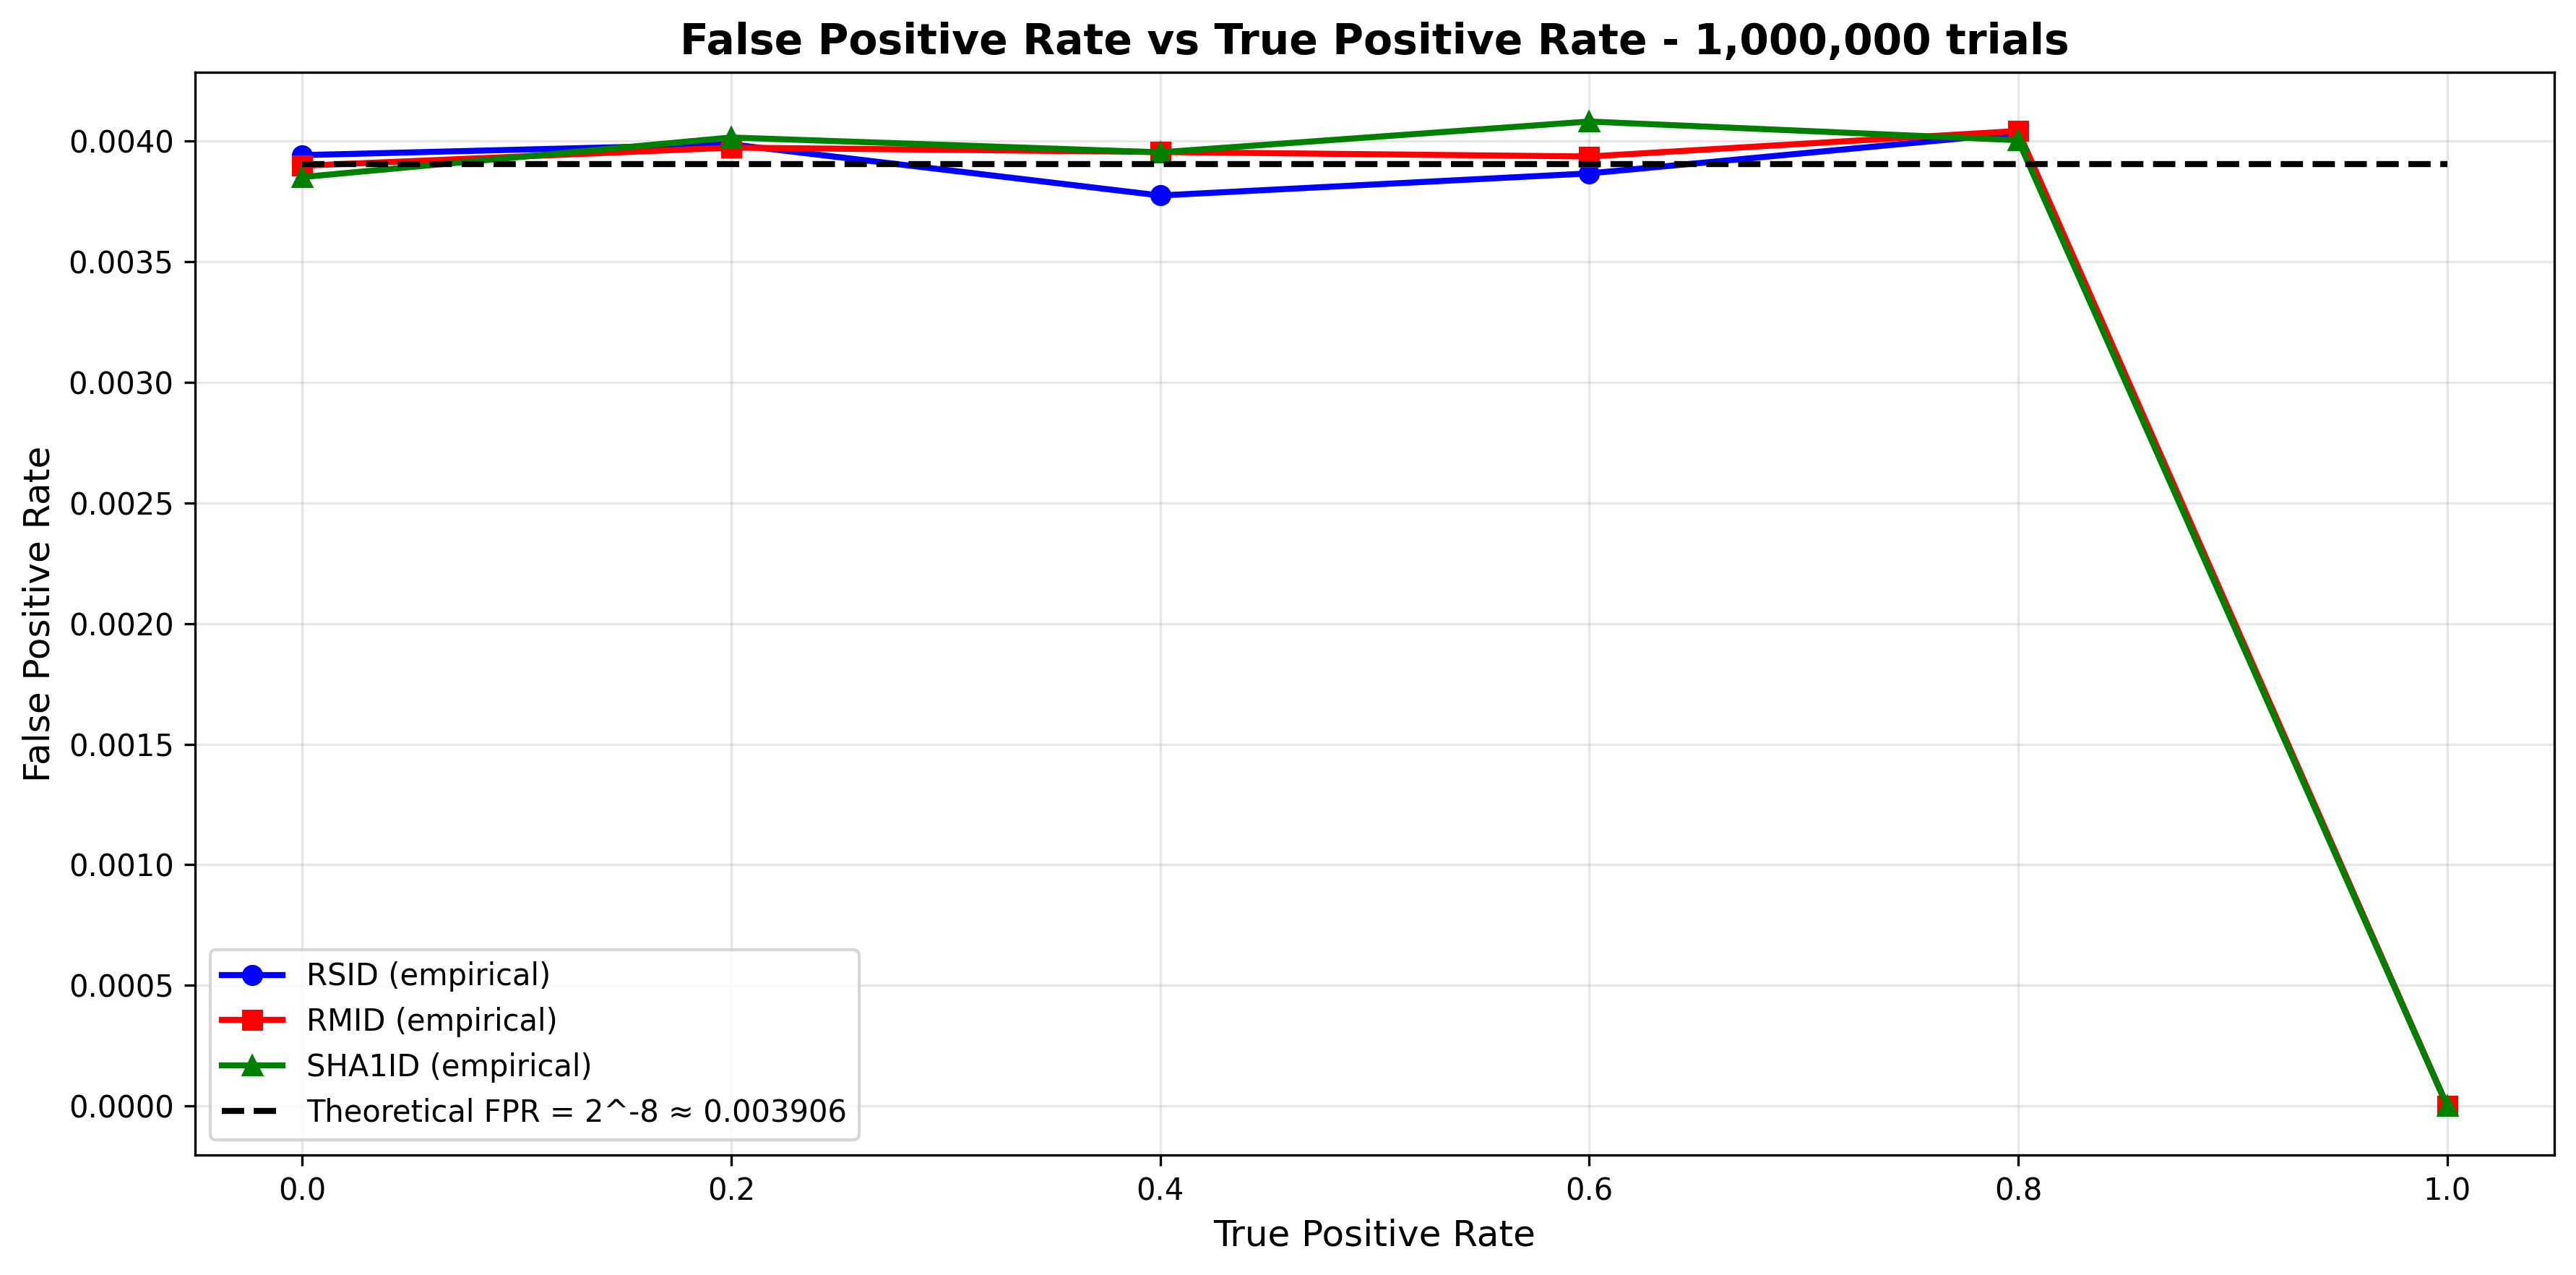
\includegraphics[width=0.75\linewidth]{plots/fpr_comparison.png}
    \caption{$\overline{p_\text{fp}}$ vs. $p_\text{tp}$ for \texttt{RSID}, \texttt{RMID} and \texttt{SHA1ID}.}
    \label{fig:fpRate}
\end{figure}

Taking a look at the mean false positive ratio $\overline{p_\text{fp}}$, defined as
\begin{equation}
\overline{p_\text{fp}} \coloneq \frac{N_\text{fp}}{N_\text{tn}} \approx \Prob(\hat{v}_p | v_n),
\end{equation}
with $N_\text{fp}$ being the number of false positive estimates $\hat{v}_\text{fp}$ by the ID-System and $N_\text{tn}$ the total number of true negatives $v_\text{tn}$.

With the property of no false negative estimates and from the above definition, it is now clear that $\overline{p_\text{fp}}$ does not depend on the true positive ratio $p_\text{tp}$. The simulation in figure \ref{fig:fpRate} shows this expected behavior, as the mean false positive ratio stays constant and is equal for all systems up until a true positive ratio of 1, where by definition the messages are always equal. This results in no false positives appearing and thus a reliability of 1. The empirical mean false positive ratio closely aligns with the theoretical value, which can be calculated regardless of the encoding scheme as the inverse of the field size $q$, as given in \cite{Codes_for_ID_Tutorial}, Sect. VI.C:
\begin{equation}
    \overline{p_\text{fp}} = \frac{1}{q} = \frac{1}{256} = 0.00390625
\end{equation}

We will now show that there is a linear relationship between $\overline{p_\text{fp}}$ and the reliability metric $r$:
\begin{align}
r &= \Prob(\hat{v}_p | v_p) + \Prob(\hat{v}_n|v_n) \\
&= \Prob(\mathbf{a} = \mathbf{b})(1 - \Prob(\hat{v}_\text{fn})) +  \Prob(\mathbf{a} \neq \mathbf{b})(1 - \Prob(\hat{v}_\text{fp})) \\
&= p_\text{tp} \cdot 1 + (1 - p_\text{tp}) \cdot (1 -\overline{p_\text{fp}}) \\
&= 1 - \overline{p_\text{fp}} + \overline{p_\text{fp}} \cdot p_\text{tp}
\end{align}
This finding aligns exactly with the empirical results in figure \ref{fig:tpRate}. Furthermore, we also get:
\begin{equation}
\frac{d(r)}{d(p_\text{tp})} = \overline{p_\text{fp}}
\end{equation}

Based on these observations, the mean false positive ratio $\overline{p_\text{fp}}$ is the underlying system property worth analysing, while the reliability metric $r$ skews the comparability of different systems because of a further degree of freedom in the true positive ratio $p_\text{tp}$.

\section{Theoretical Analysis of k-Identification}
\label{sec:kIdent}
We will now extend the metrics of interest to the k-ID scenario. Due to the fact that this variation only concerns the receiver, the code rate stays constant. Nevertheless, the error probability is effected.

As introduced in \cite{ID_Codes_Topical_Review}, "the probability of two codewords coinciding in a single symbol position is a form of the birthday problem with $q$ possible values and two participants". The statement can be generalized for k participants as the probability of at least one member of $B$ sharing the same tag as $\boldsymbol{a}$ given the condition $\boldsymbol{a} \notin B$. This can be seen as the counterprobability to the event that the tags of all elements in $B$ differ to the tag of $\boldsymbol{a}$ (similarly stated in \cite{diaconis_methods_1989}, eq. 7.1). 
Assuming that the symbols are uniformly distributed and that the tags are independent of each other, the problem yields to a collision probability of
\begin{equation}
    \Prob(t_a \in t_B | \boldsymbol{a} \notin B) = p_{\text{fp},k} = 1-\left(\frac{q-1}{q}\right)^k =  1-\left(1 - \frac{1}{q}\right)^k.\label{eq:fp prob kID}
\end{equation}
Because $p_{\text{fp},k} $ increases with k, it appears that this type of problem might not be practical. However, the actual advantage of k-ID is the decreased probability $ \mathbb{P}(\boldsymbol{a} \notin B)$ which is not reflected in this equation. 
Furthermore, the more significant probability for an overall system performance should be 
\begin{align}
    \Prob(\boldsymbol{a} \notin B | t_a \in t_B) = \frac{\Prob(t_a \in t_B | \boldsymbol{a} \notin B) \cdot \Prob(\boldsymbol{a} \notin B)}{ \Prob(t_a \in t_B)} \label{eq: P(a not in B | t_a in t_B)}
\end{align}
with the two events $\boldsymbol{a} \in B$ and $t_a \in t_B$ not independent---in contrast to the classical ID problem.
This probability \eqref{eq: P(a not in B | t_a in t_B)} can be minimized with an appropriate partitioning of the messages into subsets $B$.\\ 
For $N$ messages, equal cardinality of all $B$, fixed tag position and $n \in \NN_0$, one may consider two cases:
\begin{enumerate}
    \item $n \cdot k \cdot q = N$: This is the trivial case where a k-ID does not provide any advantage. All messages with the same tag can be grouped into one subset. This leads to the classical ID problem with a respectively less number of messages, namely $\Tilde{N} = \frac{N}{n \cdot k}$.
    \item $n \cdot k \cdot q \neq N $: For this case, the optimal classification of messages into subsets gets much more difficult and should be tailored for a specific application.
\end{enumerate}
This is where we end our investigation because a concrete partitioning should be individually adapted to the use case and has many degrees of freedom including not only the partitioning of the messages, but the relative cardinality of the subsets and the choice of the tag position as well. 

\section{Theoretical Analysis of Multiple-Tag Transmission}
\label{sec:multTag}
Our interest was to research at which cost in terms of effectiveness and code rate which gain in reliability is achievable and how this gain performs in comparison to other measures to improve reliability.

After the verification of $T$ tags, the collision probability decreases to $p_{\text{fp},T} = \frac{1}{q^T}$ since all $T$ tags have to match and identically distributed symbols are assumed.
\begin{equation}
    p_{\text{fp},T} = \prod_{i=0}^T \frac{1}{q} = \frac{1}{q^T} \label{eq: false positive probability T tags}
\end{equation}

The effective ID code rate and $T$ show a linear relationship when sending all tags at once (bulk mode) because the tag size scales linearly with $T$. Here, $R = \frac{\log(n_\text{ID})}{n_\text{cue}}$ is the ID code rate of a single tag transmission (section \ref{sec:perfId}) whereas we introduce $R_T$ as the effective ID code rate of $T$ tag transmissions. 
\begin{equation}
    R_T = \frac{\log(n_\text{ID})}{n_{\text{cue},T}} = \frac{\log(n_\text{ID})}{T \cdot n_{\text{cue}}} = \frac{R}{T}
\end{equation}
An option to keep the effective code rate at a high level is by introducing a protocol (subsequent mode): The sender sends a first tag. In the following, the receiver sends back the result of its verification estimate (one bit, c.f. $\hat{v}$ in \cite{Codes_for_ID_Tutorial}). Only if the verification has been positive, the sender sends the second tag and so on, until a maximum of $T_\text{max}$ tags have been sent. 
In this case and by using the finite geometric series, the average number $T$ of tags comprises not $T_\text{max}$, but
\begin{equation}
    T = \displaystyle \sum_{i=0}^{T_\text{max} - 1} \frac{1}{q^i} = \frac{1-q^{T_\text{max}}}{(1-q)q^{T_\text{max} - 1}}.
\end{equation}
Ideally, now the effective code rate would be
\begin{equation}
    R_T = R \cdot \frac{q^{T_\text{max} - 1}(1-q)}{1-q^T_\text{max}}.
\end{equation}
Every further tag serves as an additional assurance to prevent false positive errors. Because this is the only error type in a noiseless ID-system, the collision probability persists $p_{\text{fp},T} = \frac{1}{q^{T_\text{max}}}$.\\
For instance, if we choose $T_\text{max} = 2$, we get $p_{\text{fp},T} = \frac{1}{q^2} = \overline{p_{\text{fp}}}^2$ and $\frac{R_T}{R} =\frac{q}{1+q} \overset{q\gg1}{\approx} 1$. This shows that already for a single additional tag, the effective ID code rate approximately stagnates, whereas the collision probability squares which means that the share of false positive identification verifications is divided by the symbol size $q$ compared to the single tag case.

Regarding the false positive error bound $\lambda_{fp}^{(T)}$ with PPM-initialization, the given equation $\lambda_{fp} = \frac{K}{W}$ (\cite{ID_Codes_Topical_Review}, eq. 17) has to be extended. $K$ describes the maximum overlap of two messages, i.e. in how many positions the symbols of two different codewords are identical. $W$ is the Hamming weight and equal to the number of symbols in each codeword. Extending the transmission of a single tag, the generalized false positive error bound is
\begin{align}
    \lambda_{fp}^{(T)} &=\frac{K}{W} \cdot \frac{K-1}{W-1}\cdot ... \cdot\frac{K-T+1}{W-T+1} = \prod_{i=0}^{T-1} \frac{K-i}{W-i}\\
    &= \frac{K!}{(K-T)!} \cdot \frac{(W-T)!}{W!}\\
    &= \lambda_{fp} \cdot \frac{(K-1)!}{(W-1)!} \cdot \frac{(W-T)!}{(K-T)!}
\end{align}
for $T\leq K$ and $\lambda_{fp}^{(T)} = 0$ for $T>K$ (which again is equivalent to the transmission of the whole message).

It remains to compare the error bound of multiple small tags to the error bound of one large tag. We consider the transmission of two tags with $q = 2^8$ and the transmission of one tag with $q = 2^{16}$ so that the codeword representation stays constant. According to \eqref{eq: false positive probability T tags}, there is no difference in the collision probability. However, there is a difference in the false positive error bound ($K$, $W$ taken from \cite{ID_Codes_Topical_Review}, table 2): 

RM-PPM: $\lambda_{fp} = \frac{r}{q}$ with $K = \frac{q^m r}{q}$ and $W = q^m$ 
\begin{align}
    \lambda_{fp}^{(2)}\big|_{q=2^8} &= \frac{r}{q} \cdot \frac{q^{m-1} r -1}{q^m - 1}\\
    &(q^{m-1}r \gg 1; q^m \gg 1) \nonumber\\
    &\approx \frac{r}{q} \cdot \frac{q^{m-1} r}{q^m} = \frac{r}{q} \cdot \frac{r}{q}\\
    &\approx r\cdot \lambda_{fp}\big|_{q = 2^{16}} > \lambda_{fp}\big|_{q = 2^{16}}
\end{align}

RS1-PPM: $\lambda_{fp} = \frac{k-1}{q-1}$
\begin{align}
    \lambda_{fp}^{(2)}\big|_{q=2^8} &= \frac{(k-1)(k-2)}{(q-1)(q-2)}\\
    \frac{\lambda_{fp}^{(2)}\big|_{q=2^8}}{\lambda_{fp}\big|_{\Tilde{q} = 2^{16} = q^2}} &= \frac{(k-2)(q^2-1)}{(q-1)(q-2)} = (k-2) \cdot \frac{q^2 - 1}{q^2 -3q + 2} > 1\\
    \lambda_{fp}^{(2)}\big|_{q=2^8} & < \lambda_{fp}\big|_{\Tilde{q} = 2^{16} = q^2}
\end{align}
For both block codes, the error bound of two small tags exceeds the error bound of one large tag. In effect, one large tag provides a better reliability guarantee than two small tags. This is because a larger Galois Field spans a greater room than a small one.

\section{Test Framework Architecture}
\label{sec:testFramework}
To systematically analyze and compare ID systems under a wide range of configurations, we developed a modular Python-based evaluation framework. This framework enables automated benchmarking, statistical analysis, and interactive visualization of ID system performance. It is designed to be extensible, reproducible, and efficient, supporting both large-scale simulations and detailed metric exploration.

The framework design follows the principle of abstraction, similar to the layered approach in communication protocols like the ISO/OSI model \cite{zimmermann1980osi}. By encapsulating the specific encoding and transmission details within a well-defined ID system layer, we can focus on high-level performance metrics and treat the system under test (SUT) as a black box. This approach allows us to benefit from well-known concepts of layered design, ensuring modularity and comparability across different ID coding schemes \cite{tu2023layered}. Figure \ref{fig:frameworkArchitecture} provides a schematic overview of this architecture.

\begin{figure}[hbt!]
\centering
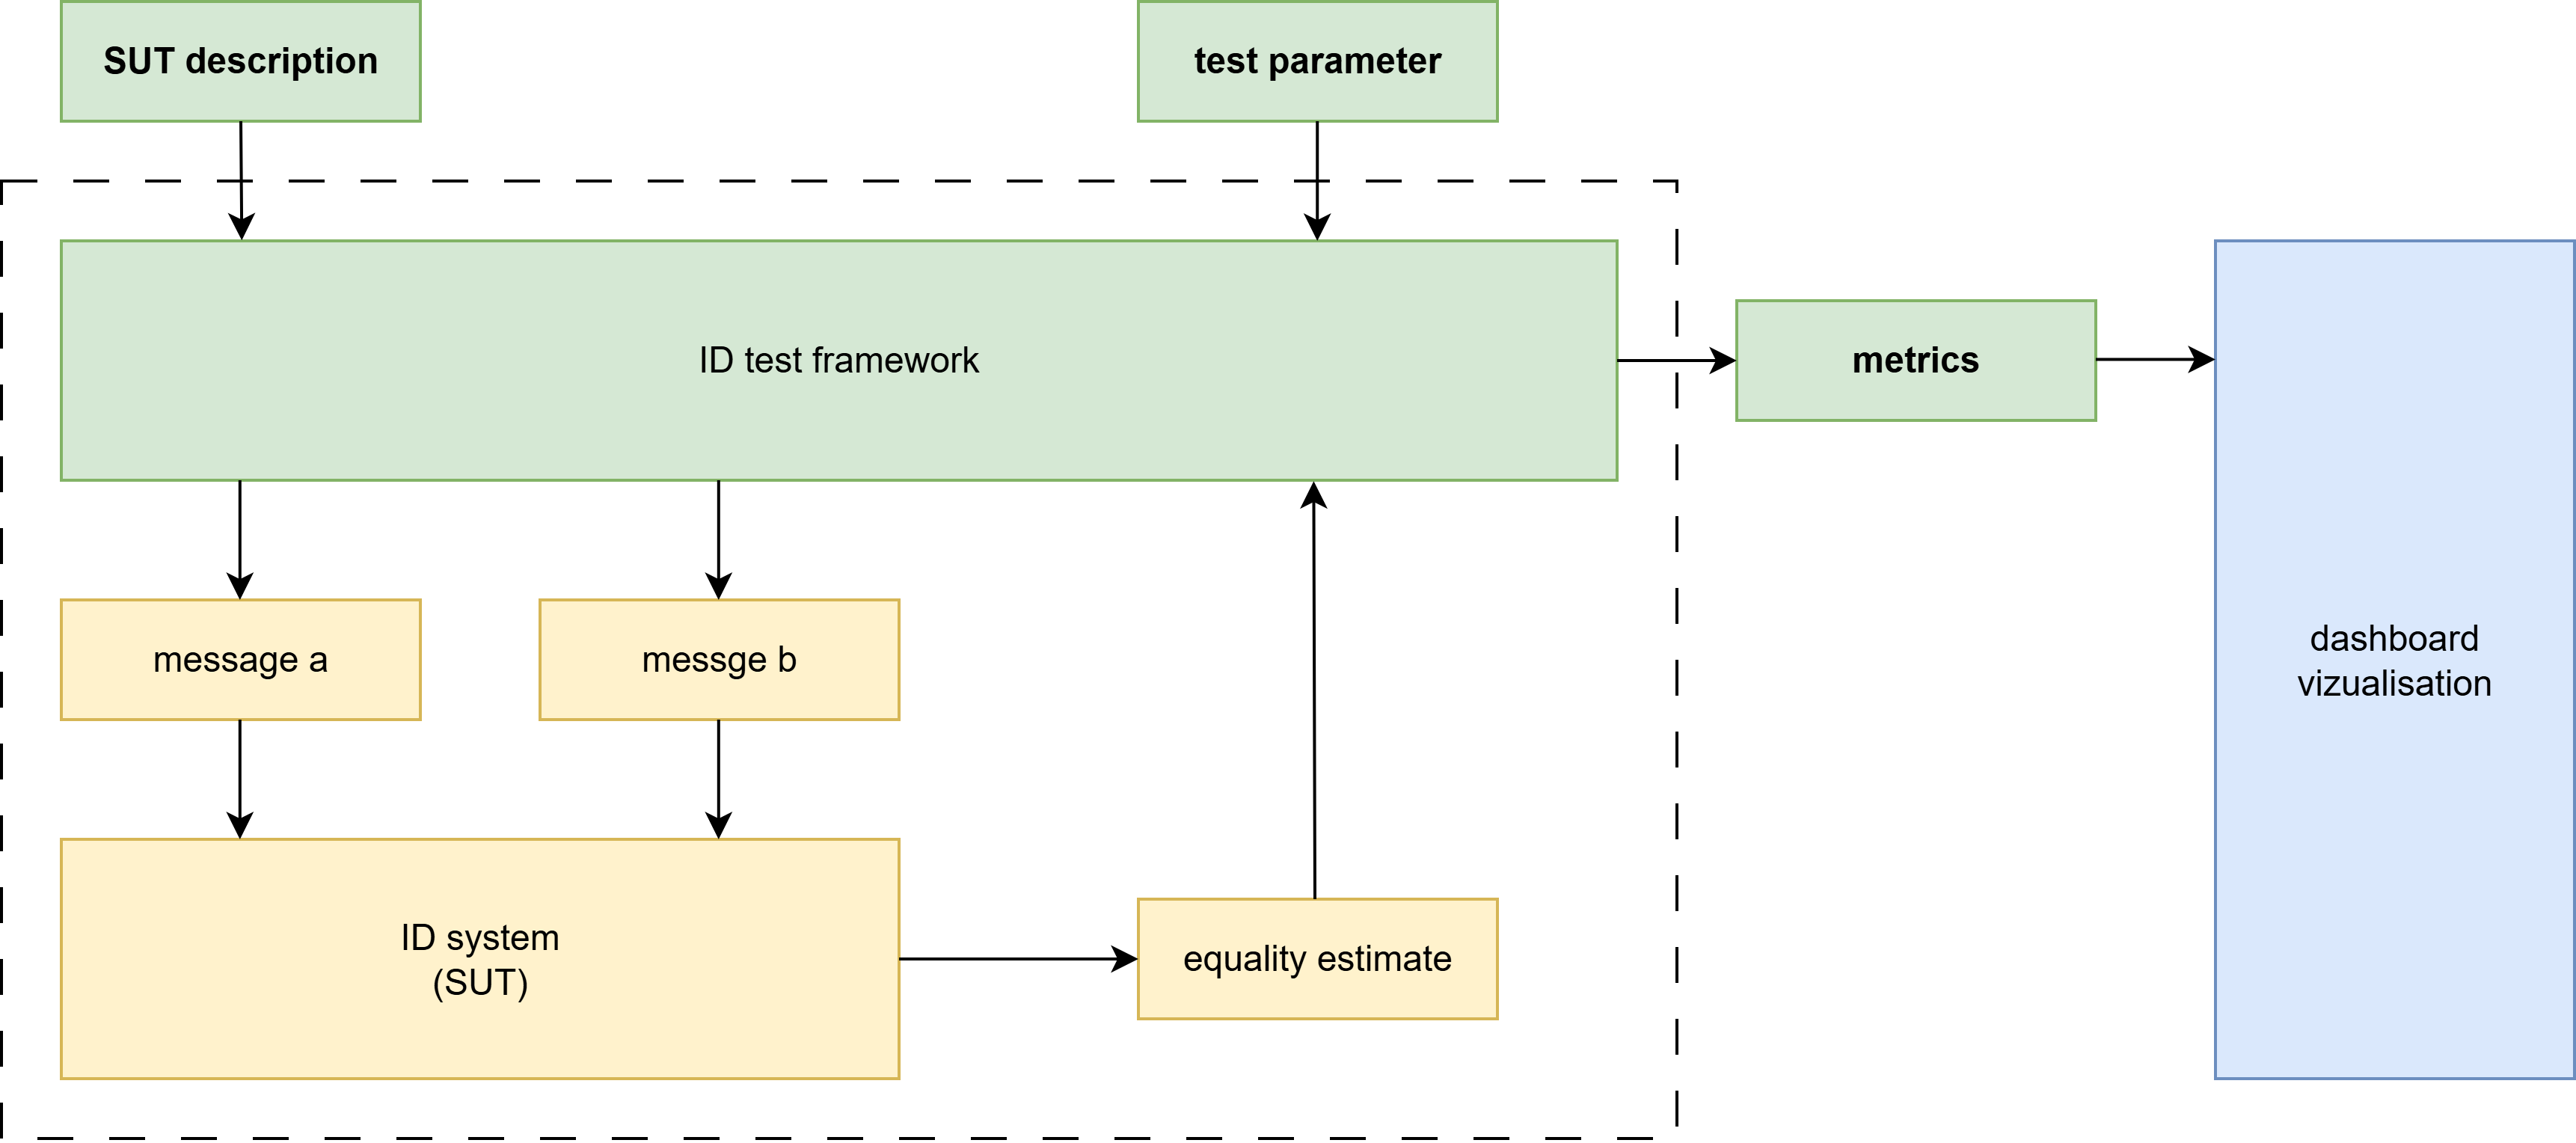
\includegraphics[width=\textwidth]{images/framework_architecture.png}
\caption{Schematic overview of the ID test framework.}
\label{fig:frameworkArchitecture}
\end{figure}

The core assumptions under which our framework operates are summarized in table \ref{tab:sysAssum}.

\begin{table}[hbt!]
\centering
\caption{System assumptions for the ID test framework.}
\label{tab:sysAssum}
\begin{tabularx}{\textwidth}{@{}lX@{}}
\toprule
\textbf{Assumption} & \textbf{Description} \\
\midrule
Noiseless channel & A noisy channel can be encapsulated by the model of a noiseless channel with different channel characteristics. It is therefore sufficient to examine a noiseless channel, keeping the option to shift to a noisy channel by concatenating with channel codes. \\
\addlinespace
No Common Randomness (CR) & The tag position remains constant for the whole test. Its influence was not examined for non-random message patterns.\\
\addlinespace
Tag position known to receiver & The tag position does not need to be transmitted because the test ID system runs on the same device. This affects metrics like the code rate. \\
\bottomrule
\end{tabularx}
\end{table}

\subsection{Core Design Principles and Abstractions}
The framework is built around several fundamental design principles that ensure scalability, maintainability, and scientific rigor. 

\textbf{Modularity and Abstraction:} At the heart of the framework lies a set of well-defined abstractions. The primary classes are an \texttt{IdEncoder} for transforming messages into tags, an \texttt{IdVerifier} for checking tag validity, and an \texttt{IdSystem} that combines both into a complete identification system. Each identification system is encapsulated as a black-box object with standardized interfaces for encoding (tag generation) and verification, allowing us to treat different coding schemes uniformly during evaluation.

\textbf{Comprehensive System Support:} The framework supports a variety of ID coding schemes, each implemented as a specialized class: Reed-Solomon-based systems (\texttt{RSID}, \texttt{RS2ID}), Reed-Muller-based systems (\texttt{RMID}), cryptographic hash-based systems (\texttt{SHA1ID}, \texttt{SHA256ID}), and a baseline \texttt{RAW} system for reference that takes a raw message symbol as the tag.

\textbf{Parameterization and Configurability:} All relevant code parameters and test conditions (e.g., message pattern, number of tags, number of validation messages) are exposed as configurable inputs. Each system is parameterizable, supporting options such as Galois field exponent (\texttt{gf\_exp}), tag positions, and code-specific parameters like Reed-Muller order. This allows for systematic exploration of the parameter space without modifying the core evaluation logic.

\textbf{Extensibility:} The modular design allows for easy extension with new coding schemes or evaluation strategies. The architecture supports the integration of new identification systems, message generators, and metrics with minimal changes to the core logic, facilitating future research directions.

\subsection{Large-Scale Parameter Sweeps and Automation}
Our experimental methodology follows a systematic multi-dimensional parameter sweep approach, evaluating ID systems across several key dimensions simultaneously.

The framework generates parameter combinations across multiple dimensions: system types (\texttt{RSID}, \texttt{RS2ID}, \texttt{RMID}, \texttt{SHA1ID}, \texttt{SHA256ID}), Galois field exponents corresponding to fields $\mathbb{F}_{2^8}$ to $\mathbb{F}_{2^{64}}$, vector lengths ranging from $2^3$ to $2^{16}$ bytes (8 to 65,536 bytes), diverse message patterns (random, sparse, low-entropy, incremental, repeated patterns), validation message counts from $2^1$ to $2^{13}$ messages for k-identification analysis, and single and multiple tag configurations where supported.

This multi-dimensional approach generates thousands of parameter combinations, requiring robust automation and fault tolerance mechanisms to handle the computational complexity effectively.

\subsection{Checkpointing and Fault Tolerance}
The framework implements a sophisticated checkpointing system that addresses the computational challenges of large-scale evaluation. This system proved essential for experiments of high computational effort, particularly when evaluating systems with large Galois fields or high message counts.

\textbf{Incremental Data Management:} Results are saved every $N$ parameter combinations (configurable), providing protection against data loss during long-running experiments. The system maintains multiple backup files to prevent data corruption and implements automatic backup creation with timestamp tracking.

\textbf{Resume Capability:} Analyses can be interrupted and resumed without data loss, allowing for flexible resource management and handling of unexpected system interruptions. The framework automatically detects existing checkpoints and continues from the last saved state.

\textbf{Progress Monitoring:} Real-time monitoring of completion percentage and estimated time remaining helps researchers plan computational resources effectively. All experimental conditions, timestamps, and metadata are recorded for each run, ensuring complete reproducibility of results.

\subsection{Performance Optimization and Parallel Processing}
Given the computational intensity of false positive rate estimation, which often requires $10^6$ to $10^7$ test messages, the framework employs several optimization strategies to manage computational resources efficiently.

\textbf{Parallel Processing:} Message generation and testing are distributed across CPU cores using worker-based parallelism. The implementation uses Python's \texttt{multiprocessing} module with careful attention to reproducibility through deterministic seeding and worker offset mechanisms.

\textbf{Memory Efficiency:} The framework implements memory-efficient statistics using online algorithms such as Welford's method for variance calculation, which is numerically stable and memory-efficient for streaming data processing \cite{Welford01081962}. Messages are processed in configurable batch sizes to balance memory usage and computational efficiency.

\textbf{Selective Computation:} Probability distribution functions are calculated only when needed to conserve memory, and the framework provides options to disable computationally expensive analyses when they are not required for specific research objectives.


\subsection{Description of Metrics}
The benchmarking process systematically explores a large parameter space. The key parameters defining the SUT and the test conditions, along with the output metrics collected, are detailed in table \ref{tab:paramDescrip}.

\begin{longtable}{@{} p{0.35\textwidth} p{0.65\textwidth} @{}}
\caption{Parameter and metric descriptions for the ID test framework.}
\label{tab:paramDescrip} \\
\toprule
\textbf{Category / Parameter} & \textbf{Description} \\
\midrule
\endfirsthead
\toprule
\textbf{Category / Parameter} & \textbf{Description} \\
\midrule
\endhead
\bottomrule
\endfoot
\bottomrule
\endlastfoot

\multicolumn{2}{@{}l}{\textbf{SUT Description}} \\
\quad system\_type & Description of the system under test. \\
\addlinespace
\multicolumn{2}{@{}l}{\textbf{Test Parameters}} \\
\quad test\_type & Type of test (e.g., execution time or false positive analysis). \\
\quad gf\_exp & Exponent of the Galois Field used in tag computation. \\
\quad vec\_len & Length of the message vector in bytes. \\
\quad tag\_pos & Position where the tag is extracted from. \\
\quad num\_tags & Number of unique tags generated. \\
\quad num\_validation\_messages & Number of validation messages in k-identification. \\
\quad num\_messages & Specified number of input messages. \\
\quad message\_pattern & Pattern for message generation. \\
\quad rm\_order & Order of the Reed-Muller code (if applicable). \\
\quad total\_messages & Total number of actually generated messages. \\
\addlinespace
\multicolumn{2}{@{}l}{\textbf{Collected Metrics}} \\
\quad false\_positive\_rate & Observed ratio of incorrect positive identifications. \\
\quad false\_positives & Absolute number of false positive detections. \\
\quad code\_rate\_bulk & Code rate in bulk message mode. \\
\quad code\_rate\_subsequently & Code rate in subsequent tag mode. \\
\quad theoretical\_fp\_rate & Theoretical false positive probability based on code parameters. \\
\quad avg\_execution\_time\_ms & Average processing time per message in milliseconds. \\
\quad std\_execution\_time\_ms & Standard deviation of execution time. \\
\quad throughput\_msgs\_per\_sec & Number of messages processed per second. \\
\quad avg\_hamming\_distance & Mean Hamming distance (HD) between messages. \\
\quad tag\_pdf & Probability distribution of tags. \\
\quad total\_analysis\_time & Total time spent analyzing all messages. \\
\end{longtable}


\section{Core Evaluation Metrics}
\label{sec:metrics_methods}
The framework implements a comprehensive suite of statistical methods to rigorously evaluate ID system performance.

The \emph{mean false positive ratio} ($\overline{p_\text{fp}}$) is a central metric, defined in (\ref{sec:sysRel}) as
\begin{equation}
\overline{p_\text{fp}} \coloneq \frac{N_\text{fp}}{N_\text{tn}} \approx \Prob(\hat{v}_p | v_n),
\end{equation}
where $N_\text{fp}$ is the number of false positive estimates and $N_\text{tn}$ is the total number of true negative cases. It quantifies the probability that a tag generated from one message is erroneously accepted as valid for a different message. In a noiseless ID system, only false positive errors can occur, as explained in Section VI.C of \cite{Codes_for_ID_Tutorial}.

Another metric is system reliability $r$, the fraction of correct identification results. It is related to the true positive ratio $p_\text{tp} \coloneq \mathbb{P}(\boldsymbol{a} = \boldsymbol{b})$ (the prior probability that sender and receiver messages are identical). As will be shown in (\ref{sec:sysRel}), $\overline{p_\text{fp}}$ is a more fundamental system property than $r$, as $r$ depends on the application-specific parameter $p_\text{tp}$. Thus, $r$ was excluded in later versions of the framework.

Execution time statistics are collected for encoding and verification operations, including average, minimum, maximum, and standard deviation. The time is measured without the framework's overhead; i.e., only the encoding time is measured through Python's \texttt{perf\_counter} method. Throughput (messages processed per second) is derived to assess computational efficiency and scalability.

To analyze the diversity of message spaces, the framework computes Hamming distance statistics between messages and between messages that produce colliding tags. Further analyses of the Hamming distance statistics were not performed in the current state of the framework, but could prove useful for evaluating the performance of the various encoders.

The framework estimates the probability mass functions (PMFs) of message and tag symbols, enabling the calculation of:
\begin{itemize}
    \item \textbf{Rényi-2 Entropy (Collision Entropy):}
    \begin{equation}
        H_2(p) = -\log_2 \left( \sum_{x \in \mathcal{X}} p(x)^2 \right) = -\log_2(p_c)
    \end{equation}
    This metric reflects the uniformity of the tag distribution and is directly related to the tag collision probability $p_c$.
    \item \textbf{Normalized Entropy Gain ($G_2$):} A metric we introduce to quantify an encoder's effectiveness in transforming a message distribution into a uniform tag distribution, bounded in $[-1, 1]$.
\end{itemize}
These metrics are crucial for evaluating performance with non-random message patterns, as detailed in \ref{sec:G_2}.

\section{Analysis of Non-Random Message Patterns}
\label{sec:nonRandom}
\subsection{Defined Message Patterns}
Thus far, analysis has often been confined to uniformly random messages, which represent an idealized scenario. To gain deeper insight into the practical performance of ID codes, we introduce several structured message patterns designed to stress the encoders in different ways. The primary goal is to establish robust metrics for a qualitative comparison of the different systems. The evaluated patterns are described in Table \ref{tab:message_patterns}.

\begin{table}[h!]
\centering
\caption{Defined message patterns for encoder evaluation.}
\label{tab:message_patterns}
\begin{tabularx}{\textwidth}{@{} lX @{}}
\toprule
\textbf{Pattern} & \textbf{Description} \\
\midrule
\texttt{random} & Messages are generated with uniformly random byte values. This serves as a baseline. \\
\texttt{incremental} & Messages consist of zeros with a final byte that increments for each new message. \\
\texttt{repeated\_patterns} & Messages consist of a short, repeating byte pattern. \\
\texttt{sparse} & Messages are mostly zeros, with a few non-zero bytes at different positions. \\
\texttt{low\_entropy} & Message symbols are drawn from a severely restricted alphabet ($\mathcal{M}=\{0,1,2,3\}$). \\
\texttt{only\_two} & Only two unique messages exist. This validates the deterministic nature of tag generation. \\
\bottomrule
\end{tabularx}
\end{table}

\subsection{Measuring Uniformity via Rényi Entropy and \texorpdfstring{$G_2$}{G2} Gain}
\label{sec:G_2}
To quantify an encoder's ability to produce the optimal uniform output distribution, we employ the Rényi entropy of order 2, also known as the collision entropy \cite{renyi1961measures}:
\begin{equation}
    H_2(p) = -\log_2 \left( \sum_{x \in \mathcal{X}} p(x)^2 \right) = -\log_2(p_c)
\end{equation}
This metric is particularly suitable for our analysis because it is directly related to the collision probability \cite{cachin1997entropy}. Maximizing the Rényi-2 entropy is equivalent to minimizing the probability of a collision. In contrast, while Shannon entropy measures the average information content \cite{The_mathematical_theory_of_communication}, it does not have this direct relationship with $p_c$. A distribution can have high Shannon entropy but still possess structural properties that lead to a higher collision probability than another distribution with slightly lower Shannon entropy, as described in \cite{renyiEntropy}.

To evaluate the effectiveness of an encoder in transforming a given message distribution ($p_M$) to a tag distribution ($p_T$) as uniformly as possible, we introduce the normalized gain metric $G_2$. This metric measures the change in $H_2$ entropy relative to the maximum possible improvement or degradation:
\begin{equation}
     G_2 = 
    \begin{cases}
        \frac{H_2(p_{T}) - H_2(p_{M})}{H_2^{\text{gain}}}, &  H_2(p_{T}) \ge H_2(p_{M}) \\
        \frac{H_2(p_{T}) - H_2(p_{M})}{H_2^{\text{loss}}}, &  H_2(p_{T}) < H_2(p_{M})
    \end{cases}
\end{equation}
where the maximum possible entropy gain is $H_2^{\text{gain}} = \log_2(|\mathcal{T}|) - H_2(p_M)$ (the difference between maximum and initial entropy), and the maximum possible loss is $H_2^{\text{loss}} = H_2(p_M)$ (the difference between initial and minimum entropy, which is 0).

The maximum possible entropy gain corresponds to the Rényi divergence of the second order $D_2(P\|Q)$ \cite{van_Erven_2014}, defined as: 
\begin{equation}
    D_2(P\|Q) = \log_2 \sum_{i=1}^n \frac{p_i^2}{q_i}
\end{equation}
from a uniform tag distribution with probability mass function $u$. Let the alphabet be $\mathcal{M} \subseteq \mathcal{T}$. In our case:
 \begin{align}
     D_2(p_M\|u) &= \log_2 \sum_{i=1}^{|\mathcal{T}|} \frac{p_M^2(i)}{1/|\mathcal{T}|} \\
     &= \log_2 ( |\mathcal{T}| \sum_{i=1}^{|\mathcal{T}|} p_M^2(i)) \\
     &= \log_2 (|\mathcal{T}|) - H_2(p_M) \\
     &= H_2^{gain}
 \end{align}
Similarly, the maximum possible entropy loss is derived by considering a transformation to a deterministic distribution, which has the minimum possible entropy. A deterministic distribution $p_{\text{det}}$ has a probability of 1 for a single outcome and 0 for all others. Its Rényi-2 entropy is:
 \begin{align}
     H_2(p_{\text{det}}) &= -\log_2 \left( 1^2 + \sum_{i=1}^{|\mathcal{T}|-1} 0^2 \right) \\
        &= -\log_2(1) = 0
 \end{align}
With this insight, we can interpret the $G_2$ metric as a type of statistical distance, bounded in $[-1, 1]$. A positive value indicates a gain in uniformity (lower $p_c$), while a negative value signifies a loss (higher $p_c$). A score of $G_2 = 1$ denotes a perfect transformation to a uniform distribution, whereas $G_2 = -1$ represents a collapse to a deterministic output with maximum collision probability.

\section{Interactive Visualization Dashboard}
\label{sec:metVis}
To visualize the analysed metrics, a variety of variables must be considered that influence the behavior of the ID system. The interactive dashboard provides users with a comprehensive overview, allowing them to examine and compare the behavior of different encoders. Multiple ID systems can be displayed side by side to enable direct comparison. In addition, the dashboard facilitates the recognition of optimal configurations as well as the advantages and disadvantages of various systems.

\subsection{k-Identification Panel}
The first panel of the dashboard displays the false positive ratio (c.f. \ref{sec:sysRel}) obtained in k-Identification (\ref{sec:kIdent}) using various encoders. It is shown in figure \ref{fig:dashKID}. On the left-hand side, all available controls for the relevant variables are located. The user can first select two different encoders to be compared. Depending on the available dataset, several additional options appear below. Among these is the ability to select the Galois Field exponent used for symbol representation in the messages. Further options relate to the message pattern, as explained in more detail in section (\ref{sec:mesPat}). If either \texttt{RMID} or \texttt{RSID} is selected, an additional parameter appears, allowing the user to set the number of tags, corresponding to the scenario discussed in sections (\ref{sec:VerIdprob}) and (\ref{sec:multTag}).

Once all parameters are selected, the central graph visualizes the false positive ratio as a function of the number of validation messages. For reference, a theoretical bound \eqref{eq:fp prob kID} is also displayed to allow for better comparison. If the false positive ratio reaches zero, an appropriate notification is shown below the graph. The axes are scaled logarithmically on both sides (log-log scale) to ensure that all data points are clearly visible and to reveal exponential dependencies in the results. On the right-hand side of the panel, the ID code rates of the selected systems are shown, along with information about the tag transmission rules.

\subsection{Execution Time Panel}
The second panel in figure \ref{fig:dashExecTime} displays the execution time in relation to the vector length of the observed messages. The same control elements as in the first panel are available for selecting encoder types and other relevant parameters. Two diagrams are shown: one for execution time and one for throughput, both using log-log scaling. In this representation, the axis ranges are fixed to enable consistent comparison, even when the input parameters are changed.

\subsection{System Comparison Panel}
The next panel in figure \ref{fig:dashSysComp} also displays information about execution time and throughput. However, in contrast to the previous panels, all system types are shown simultaneously using bar charts. This allows a direct comparison of all systems at once. The vector length can be adjusted using the slider below the diagrams. For \texttt{RMID} and \texttt{RSID}, the option to select different numbers of tags is again available. Ideally, the y-axes of the bar charts would use a fixed scale to ensure consistent comparison. However, this is not feasible in practice, as very small values would become nearly invisible, which would significantly reduce the clarity and readability of the visualization.

\subsection{PMF Visualization Panel}
The panel for the probability mass function (PMF) in figure \ref{fig:dashPMF} serves as a visual supplement to the explanations provided in section (\ref{sec:mesPat}). Users can select any combination of encoder and symbol distribution. The graphic on the right visualizes the values of the message symbols, using different colors for distinction. Below this, the diagram on the left displays the corresponding PMF of the message symbols. The diagram on the right shows the PMF of the generated tag. The significance of these distributions and their implications are discussed in detail in section (\ref{sec:mesPat}).


\chapter{Results and Discussion}
\label{chap:evalInter}

\section{Analysis of Non-Random Message Patterns}
\label{sec:mesPat}
Table \ref{tab:G2} summarizes the $G_2$ scores (\ref{sec:G_2}) from our simulations. The \texttt{only\_two} pattern, being a consistency check, is excluded from the mean calculation. As a reference, the \texttt{RAW} system does not apply any ID-Code, but rather chooses a message symbol at a fixed position as the resulting tag.

\begin{table}[hbt!]
\centering
\caption{Rényi-2 Entropy Gain ($G_2$) for Various Encoders and Message Patterns.}
\label{tab:G2}
\begin{tabular}{@{}lrrrrrr@{}}
    \toprule
    \textbf{Pattern/System} & \textbf{RAW} & \textbf{RSID} & \textbf{RS2ID} & \textbf{RMID} & \textbf{SHA1ID} & \textbf{SHA256ID} \\
    \midrule
    \texttt{random}         & -3.97e-06 & -4.13e-06 & -4.36e-06 & -4.15e-06 & -4.41e-06 & -4.63e-06 \\
    \texttt{incremental}    & -1.0000   & 0.9993    & 0.8717    & -1.0000   & 0.8652    & 0.8813 \\
    \texttt{repeated}       & -1.25e-05 & -0.0192   & -0.0243   & -0.1572   & -0.0302   & -0.0262 \\
    \texttt{sparse}         & -0.0020   & 0.9960    & 0.9944    & 0.1057    & 0.9944    & 0.9932 \\
    \texttt{low\_entropy}   & -9.21e-08 & 1.0000    & 1.0000    & 0.1667    & 1.0000    & 1.0000 \\
    \midrule
    \textbf{Mean}           & \textbf{-0.2004} & \textbf{0.5952} & \textbf{0.5684} & \textbf{-0.1770} & \textbf{0.5659} & \textbf{0.5697} \\
    \bottomrule
\end{tabular}
\end{table}

\textbf{Random:} With a uniformly random input, all systems perform as expected, showing a $G_2$ value approximately zero. This confirms they do not degrade an already optimal distribution.

\textbf{Incremental:} This pattern, with its limited space of 256 unique messages, reveals significant differences in how encoders handle highly structured, low-entropy input. The \texttt{RAW} system performs worst ($G_2 = -1.0$), as the tag is extracted from a fixed position that is always zero. This results in a constant output tag, minimizing the output entropy.

Conversely, Reed-Solomon codes (\texttt{RSID} and \texttt{RS2ID}) are designed to handle burst errors, which is analogous to this input pattern. As linear block codes over the finite field $\mathbb{F}_{2^8}$, their output codeword $\mathbf{c}$ is a linear transformation of the input message vector $\mathbf{m}$: $\mathbf{c} = \mathbf{m}G$ \cite{macwilliams1977theory}, where $G$ is the $k \times n$ generator matrix. For messages of the form $\mathbf{m}_i = [0, 0, \ldots, 0, i]^\intercal$, where $i \in \mathbb{F}_{2^8}$, the linearity of the code implies that the codeword is $\mathbf{c}_i = i \cdot \mathbf{g}_{k}$, where $\mathbf{g}_{k}$ is the last row of $G$. A tag taken from a fixed position $\pi$ of the codeword is $t_i = i \cdot g_{k, \pi}$, where $g_{k, \pi}$ is a fixed, non-zero constant from the generator matrix. The operation is multiplication in $\mathbb{F}_{2^8}$. As the input $i$ cycles through all 256 elements of $\mathbb{F}_{2^8}$, the output $t_i$ also cycles through all 256 unique elements, because multiplication by a non-zero element in a finite field is a permutation \cite{lidl1997finite}. This creates a perfectly uniform tag distribution. \texttt{RSID} exhibits this theoretical behavior ($G_2 \approx 1.0$), demonstrating its ideal suitability for this pattern. The slight deviation from a perfect score is attributed to the simulation logic for false positives, which omits one possible message-pair, thus leaving one tag value ungenerated.

The concatenated \texttt{RS2ID} code shows good but slightly degraded performance ($G_2 \approx 0.87$). The outer RS code operates on symbols from an extension field $\mathbb{F}_{q^{k_i}}$. The incremental message pattern provides a very sparse set of inputs to this outer encoder. This sparse input set is mapped to a sparse set of output symbols in the extension field (figure \ref{fig:rsid_16_pmf}). When these symbols are expanded back to bytes and a tag is selected from a fixed inner position, the resulting distribution is non-uniform, appearing as a comb-like PMF where many possible tag values are never generated. This structural artifact slightly reduces the output entropy.

Reed-Muller (\texttt{RMID}) codes perform exceptionally poorly ($G_2 = -1.0$). RM codes operate on bits, and the codeword is the evaluation of a Boolean polynomial whose coefficients are the message bits \cite{muller1954application}. In this pattern, only the 8 bits of the final byte ever change. It is likely that the specific basis polynomials corresponding to these 8 bits evaluate to zero at the chosen, fixed output coordinate used for the tag. Consequently, the tag's value is determined only by the static (all-zero) part of the message, making the tag constant and maximizing collision probability.

The cryptographic hashes (\texttt{SHA1ID}, \texttt{SHA256ID}) perform well due to their strong diffusion properties, often called the avalanche effect, which ensures that small changes in the input lead to pseudo-random, unpredictable changes in the output \cite{menezes1996handbook}.

\textbf{Repeated Patterns:} With the exception of \texttt{RAW}, all coding schemes show a negative $G_2$ score, meaning they increase the collision probability compared to the input. This is a critical finding: while these encoders scramble the input, their fixed algebraic structure can interact unfavorably with the input's regularity. This creates unexpected collisions, where distinct-but-structured input messages map to the same output tag. This phenomenon highlights a failure of these specific codes to adequately break the input pattern's structure, a weakness directly captured by the Rényi-2 entropy metric.

\textbf{Sparse:} The \texttt{RAW} system has a $G_2 \approx 0$ because both the input message distribution and the output tag distribution have very low entropy. The output tag is almost always zero, unless a non-zero byte happens to be placed at the specific tag-sampling position. Since there is little change between the low-entropy input and the low-entropy output, the gain is near zero. \texttt{RSID}, \texttt{RS2ID}, and the SHA-based systems again show excellent performance, effectively diffusing the sparse non-zero inputs across the output space. \texttt{RMID}'s gain is muted because the high number of zero bits in the input message vector results in a sparse polynomial with limited output variability.

\textbf{Low Entropy:} When drawing from the restricted alphabet $\mathcal{M}=\{0,1,2,3\}$, all encoders except \texttt{RMID} achieve a near-perfect $G_2 \approx 1.0$. \texttt{RMID}'s performance is severely hampered because it operates bit-wise. The message symbols (binary `00000000` to `00000011`) ensure the six most significant bits of every message byte are always zero. If these bits correspond to the coefficients of low-degree, high-influence basis polynomials, their constant zero value will heavily bias the output, preventing a uniform tag distribution.

\textbf{Only Two:} This pattern served as a consistency check for determinism. For all systems, the input and output distributions consist of two equiprobable symbols.

\section{k-Identification: Results and Discussion}
\label{sec:FindingskID}
Theoretically, a k-ID scenario increases the error metrics of an ID system (section \ref{sec:kIdent}). In spite this pessimistic conclusion, the statement may not represent a positive influence on the whole system when the messages are grouped effectively. Therefore, an evaluation of the complete scenario has to take the concrete partitioning into consideration. Furthermore, the semantic meaning of a message, thus the mapping of interpretation to a bit sequence, influences the partitioning as well. This seems to be the main task when k-ID is established and must be tailored to the specific application. 

On the other hand, one must raise the question if the quantization of messages into subsets at the receiver was practical or if it would be more efficient to undergo this step in the sender before the tag computation. The only case when it could be favorable to use this kind of ID is with changing or apriori unknown message subsets $B$, whereat the optimal partitioning of messages is even more difficult because all possible constellations have to be taken into consideration.

When we regard the simulation results, due to limitations in computational resources, some metrics indicate that the false positive ratio remains consistently zero. This occurs in all simulations using a Galois field exponent greater than or equal to 32, with the exception of the \texttt{RMID} encoder combined with the low\_entropy pattern. In this specific case, the observed false positives reflect the comparatively poor performance of the \texttt{RMID} encoder under these parameters. For the other ID systems, obtaining meaningful results would require a significantly larger number of simulation runs with more validation messages to observe even a single false positive event. This was beyond the scope of our available resources; therefore, no further analysis was conducted in these cases.

If the selected message pattern is set to random, the symbols in the simulated messages follow a uniform distribution. As a result, the encoded tags also exhibit a uniform distribution. This behavior is illustrated in the PMF panel. A uniformly distributed tag is also assumed in the theoretical derivation of the false positive rate bound as mentioned in Section VI. C of \cite{ID_Codes_Topical_Review}. Consequently, the corresponding graphs are expected to align closely with this bound. This pattern is confirmed by the \texttt{RMID} and the \texttt{RSID} systems shown in the figure \ref{fig:fpratioRandom}.

\begin{figure}[!t]
    \centering
    \includesvg[width=0.75\linewidth]{plots/fpratio_rmid_rsid_random_1tag_gf16}
    \caption{$fp\_ratio$ vs. $num\_val\_msg$ for \texttt{RMID} and \texttt{RSID} with the random message pattern, num\_tags = 1, gf\_exp = 16} 
    \label{fig:fpratioRandom}
\end{figure}

The \texttt{SHA1ID} and \texttt{SHA128ID} encoders exhibit nearly identical performance. Their results consistently lie very close to the theoretical bound. Since these encoders can only be simulated with a single tag, no further variation or analysis is applicable.

\section{Multiple-Tag Scenarios: Results and Discussion}
\label{sec:FindingsMultiTag}

Regarding the transmission of multiple tags (section \ref{sec:multTag}), the ID code rate decreases linearly, the average collision probability decreases exponentially and the false positive error bound decreases linearly with the number of tags. With the introduction of a subsequent transmission of tags, the ID code rate even decreases less than linearly. This means that the reliability can be increased significantly with almost no effect on the code rate. 
The behavior is reflected in the dashboard by the slower decrease of the code rate in subsequent transmission mode compared to bulk transmission, as the number of tags increases. However, the receiver's answer and signal processing require additional overhead. This entails propagation and processing delay as a result of the  transmission as well as channel coding of the estimate. In addition, a feedback channel is needed and possibly requires further hardware equipment on both sides.
Consequently, the effective ID code rate will not reach its optimum, but still stays at a high level.

%In another scenario, the effect of different tag transmission rules on the ID code rate is examined. In the so-called subsequent transmission mode, the number of transmitted tags is not fixed in advance. Additional tags are only sent if the receiver provides positive feedback indicating that the messages could be equal. Consequently, in the case of a false positive, the maximum number of tags is transmitted. However, if a true negative occurs, it is likely that only one tag is sent. Since fewer tags are transmitted on average, the code rate improves in comparison to the bulk mode, in which all tags are sent at once. 

%However, this gain comes at the cost of requiring a feedback channel from the receiver to the sender, which introduces additional technical complexity. 

The transmission of one large tag is more reliable than the transmission of two small tags with constant overall tag size. Thus, the transmission of multiple tags has a lower performance regarding reliability. On the other hand, because the ID code rate is higher, it might be an option if the code rate appears to be more important.

To examine the false positive ratio with respect to the number of transmitted tags, the results align precisely with the statement made in Section VII. D of \cite{Codes_for_ID_Tutorial}:

\begin{quote}

"[...] However, each additional tag reduces the mean collision probability by a factor $\frac{1}{q}$, thus improving reliability." 
 
\end{quote}

This relationship is confirmed by the behavior of the \texttt{RSID} system shown in figure \ref{fig:tagCompare}. Its graph closely follows the theoretical bound, clearly demonstrating the expected decrease in failure probability and validating the predicted $\frac{1}{q}$ reduction with each additional tag. The \texttt{RMID} system also shows a decreasing false positive ratio as the number of tags increases. However, its performance is significantly weaker compared to the \texttt{RSID} system, as its results deviate substantially from the theoretical values.

The code rate metrics can be further analyzed by varying the Galois field exponent. It directly determines the size of a single message symbol, and thus the size of each tag. As a result, increasing the Galois field exponent reduces the ID code rate, since more bits are required to represent the same message. This relationship is clearly visible in the dashboard and is also discussed in Section VII.B of \cite{Codes_for_ID_Tutorial}. 

\begin{figure}[htbp]
  \centering
  \begin{minipage}[t]{0.32\textwidth}
    \centering
    \includesvg[width=\linewidth,inkscapelatex=false]{plots/1:q_proof_1tag}
    \caption{t = 1}
  \end{minipage}
  \hfill
  \begin{minipage}[t]{0.32\textwidth}
    \centering
    \includesvg[width=\linewidth,inkscapelatex=false]{plots/1:q_proof_2tag}
    \caption{t = 2}

  \end{minipage}
  \hfill
  \begin{minipage}[t]{0.32\textwidth}
    \centering
    \includesvg[width=\linewidth,inkscapelatex=false]{plots/1:q_proof_3tag}
    \caption{t = 3}

  \end{minipage}
  \caption{Relation of ID systems to average error for different numbers of tags t, gf\_exp = 8, low\_entropy}
  \label{fig:tagCompare}
\end{figure}



\section{Execution Time Analysis}
\label{sec:exectime}
The dashboard panels for execution time versus vector length and system comparison provide insights into the performance of both the encoders and the overall framework. Since all systems exhibit a similar general trend, a focused analysis of two representative encoders is sufficient to draw basic conclusions about the overall performance. For this purpose, the \texttt{RSID} and \texttt{SHA1ID} encoders were selected, as their behavior is very similar.

\begin{figure}[h!]
    \centering
    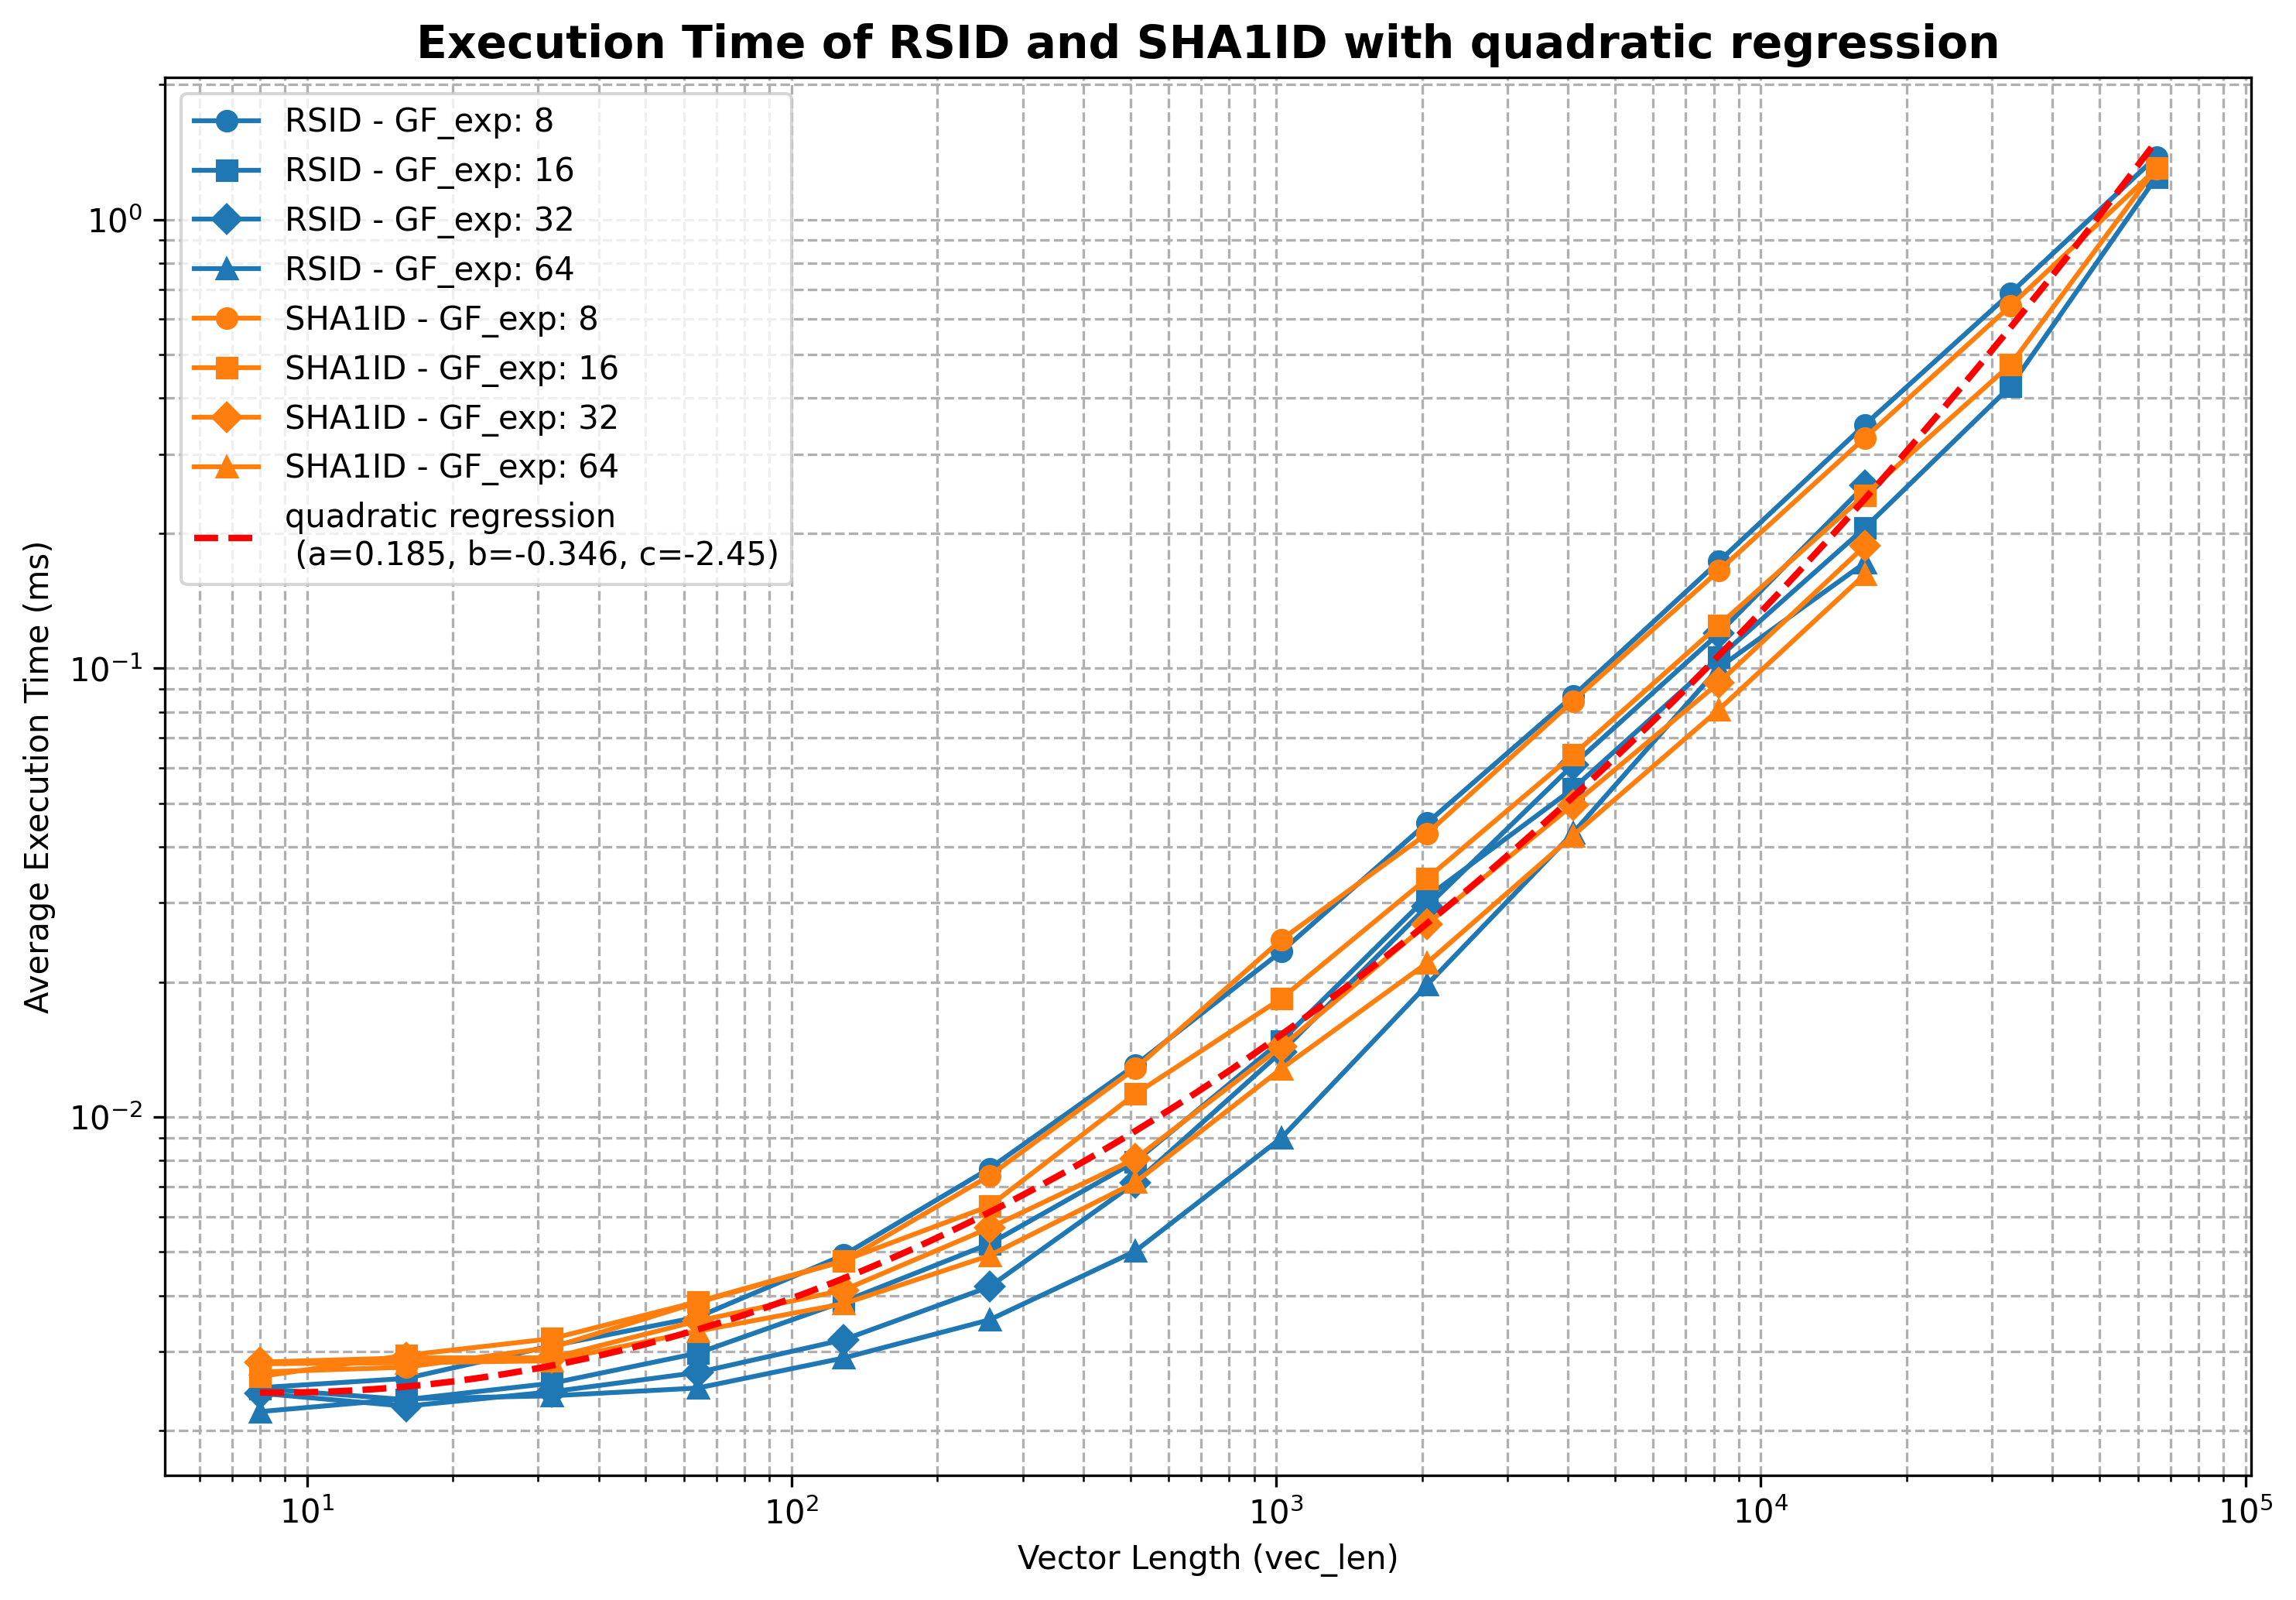
\includegraphics[width=0.75\linewidth]{plots/execution_time_quadratic_regression.png}
    \caption{Execution time vs. vector length for \texttt{RSID} and \texttt{SHA1ID} with a quadratic regression in log-log space.}
    \label{fig:quadRegExec}
\end{figure}

Figure \ref{fig:quadRegExec} shows their performance across different Galois field exponents. A clear upwards trend is visible in the graphs. To investigate this trend further, a quadratic regression was performed using the following formula:
\begin{align*}
     \log_{10}(y) = \boldsymbol{a} \cdot \left( \log_{10}(x) \right)^2 + \boldsymbol{b} \cdot \log_{10}(x) + \boldsymbol{c}
 \end{align*}
 For the calculation, the Python library $NumPy$ was used, specifically the $polyfit$ method. This method applies the least squares approach, as described in \cite{leastSquareProblems}. It yielded the following coefficients:
 \begin{align*}
     \boldsymbol{a} = 0.185 \quad \boldsymbol{b} = -0.346 \quad \boldsymbol{c} = -2.45
 \end{align*}
These values must be further examined in the context of a log-log plot. The most relevant parameter for assessing scalability to larger vector lengths is the coefficient $\boldsymbol{a}$. If a is greater than zero, the curve in the log-log plot bends upward, indicating a convex shape. This behavior suggests a more than polynomial relationship between vector length and execution time. While the detailed mathematical implications of such functions are beyond the scope of this report, it can be concluded that this trend implies poor performance of both the encoders and the framework for very large datasets. The other coefficients, $\boldsymbol{b}$ and $\boldsymbol{c}$, provide information about performance at smaller vector lengths. A low $\boldsymbol{c}$ value indicates low execution times for the shortest vectors, while a negative $\boldsymbol{b}$ suggests a slow initial growth of the curve, which reflects good performance for smaller input sizes. This matches the curve of the simulation data.

The execution time graphs of the other systems follow a relatively similar trend. Although this regression is a simplified approach to describe the behavior at larger vector lengths, it effectively illustrates a general issue: increasing vector sizes lead to significantly higher computation times, a challenge common to all systems.


\chapter{Summary and Outlook}

\section{Summary}
\label{sec:summary}
This report details the evaluation of ID systems, specifically focusing on noiseless ID tagging codes, within the scope of the \textit{Hauptseminar Kommunikationssysteme}. Our primary objective was to gain an intuitive understanding of ID system behavior under various configurations and to assess their practical performance. We confirmed existing theoretical trends found in relevant literature \cite{ID_Codes_Topical_Review} while also extending the evaluation to several novel scenarios not extensively covered before. These include transmitting multiple tags, operating within a k-Identification context, and analyzing performance with diverse non-random message patterns. The insights were facilitated by a developed test framework and an interactive dashboard for metric visualization, which served as crucial tools throughout the analysis.

Key findings from our extended investigations are summarized as follows:

Firstly, in the \textbf{k-Identification scenario} (section \ref{sec:kIdent}), where the receiver aims to determine if its message matches any in a set of $k$ possible messages, we derived the mean false positive ratio as $1-(1-\frac{1}{q})^k$. While this probability theoretically increases with $k$, the actual advantage of k-ID lies in the potential for a significantly decreased prior probability that the sender's message is not in the receiver's set. The main challenge, however, is determining an optimal strategy for grouping messages into advantageous subsets, which is highly dependent on the specific application's semantic interpretation of messages. If implemented effectively, k-ID systems have the possibility to contribute to a more relaxed overall reliability requirement for certain applications.

Secondly, concerning \textbf{multiple tag transmission} (section \ref{sec:multTag}), we found that increasing the number of transmitted tags significantly enhances reliability by exponentially reducing the mean false positive ratio ($p_{\text{fp},T} = \frac{1}{q^T}$). While transmitting two smaller tags can achieve the same mean false positive ratio as one larger tag (with an equivalent total message representation), one large tag consistently offers a lower superior false positive error bound, thus providing a stronger reliability guarantee. Furthermore, we analyzed the impact on the ID code rate, observing a linear decrease in bulk mode (all tags sent at once) versus a less-than-linear decrease in subsequent mode (tags sent conditionally upon receiver feedback). The latter mode offers improved code rates at the expense of requiring a feedback channel and introducing additional protocol overhead. This highlights a tunable trade-off between desired reliability and code rate for system designers. 

Thirdly, our analysis of \textbf{non-random message patterns} (section \ref{sec:mesPat}) provided crucial insights into the performance of different encoding schemes beyond the idealized assumption of uniformly random messages. We leveraged Rényi-2 entropy (collision entropy) and a novel $G_2$ gain metric to quantify an encoder's ability to transform diverse message input distributions into a uniform tag distribution, which is optimal for minimizing collision probability. This approach proved more appropriate for collision-sensitive ID systems than traditional Shannon entropy. We found that Reed-Solomon (\texttt{RSID}, \texttt{RS2ID}) codes consistently demonstrated superior performance, often closely approximating a uniform tag distribution due to their inherent algebraic properties. Cryptographic hash functions (\texttt{SHA1ID}, \texttt{SHA256ID}) also exhibited excellent diffusion capabilities. In contrast, Reed-Muller (\texttt{RMID}) codes often showed limitations, particularly for highly structured or low-entropy inputs. A significant conclusion was that simply scrambling an input to increase its Shannon entropy does not necessarily guarantee a reduced collision probability; instead, specific attention to the uniformity of the tag distribution is paramount for ID systems.

Finally, practical considerations regarding \textbf{execution time} (section \ref{sec:exectime}) revealed a more than polynomial growth with increasing message vector length across all evaluated systems. While this indicates scalability challenges for exceptionally large datasets, the framework still proved effective for investigating behavior within relevant practical ranges. It became apparent that empirically validating the theoretical (and often minuscule) false positive ratios or bounds, especially for higher Galois Field exponents or multiple tags, demands immense computational resources beyond the scope of this project. Even for small field sizes, observing rare false positives required sending millions of messages. This limitation reinforces the importance of the theoretical error probability bounds for guaranteeing reliability in safety-critical applications, as these provide assurances where empirical observation might be impractical.

In essence, our report confirmed theoretical foundations of noiseless ID systems, extended the understanding of their performance in various practical scenarios, highlighted key trade-offs in their design, and underscored the importance of tailored metrics for evaluating their effectiveness.

    
\section{Limitations and Outlook}
\label{sec:outlook}
It is important to note that with our probabilistic test setup, we soon reached the limits of our ability to validate theoretical values. Further optimizing the code parameters, e.g., using multiple tags (section \ref{sec:multTag}), made the main investigated metric of false positives decrease to minuscule values, such that the number of necessary test messages reached enormous amounts. In spite of small field sizes, like $\mathbb{F}_{2^{16}}$, and with $10^7$ sent messages, we only ever observed 316 false positives using a simple \texttt{RSID} tagging encoder. For larger fields like $\mathbb{F}_{2^{32}}$ or $\mathbb{F}_{2^{64}}$, we were not able to observe false positives in any configuration. Even with advanced techniques like parallel computing and batch processing, the rare event testing as done in this report remains a time consuming procedure.

It could be the subject of further investigations to apply various test setups on the ID problem to still ensure reliable system evaluation, but with reduced computational effort.
Boundary testing, where codewords are designed and tags are chosen specifically to test edge cases, seems to be a promising alternative to the probabilistic approach of this report \cite{dobslaw2020boundary}. Similar to the approach used in section \ref{sec:mesPat}, codes and tags can be divided into groups of similar patterns, analogue to grouping messages (k-ID, section \ref{sec:kIdent}). Facing the challenge of eliminating unnecessary test cycles, codes and tags that are marked as unproblematic could be filtered out. Keeping only combinations that are likely to cause a false positive identification enables a reduction of computational and time efforts.   

Nevertheless, one should keep in mind that a main advantage of the evaluated ID codes is that their characteristic of having a defined error probability can barely be demonstrated nor proven in a probabilistic demo like the one in this report. An error probability bound (c.f. \cite{Codes_for_ID_Tutorial}, Section VII.C) is what ensures safety and what makes it suitable even for safety-requiring applications, e.g., digital twins \cite{von_lengerke_identification_2023}. 


\vspace{1cm}

\printbibliography


\appendix
\chapter{Appendix}

\begin{figure}[hp]
  \centering
  \includesvg[width=\textwidth]{plots/pmf's/pdf_incremental.svg}
  \caption{PMF for incremental pattern.}
  \label{fig:incremental}
\end{figure}

\begin{figure}[hp]
  \centering
  \includesvg[width=\textwidth]{plots/pmf's/pdf_low_entropy.svg}
  \caption{PMF for low entropy pattern.}
\end{figure}

\begin{figure}[hp]
  \centering
  \includesvg[width=\textwidth]{plots/pmf's/pdf_only_two.svg}
  \caption{PMF for only two pattern.}
\end{figure}

\begin{figure}[hp]
  \centering
  \includesvg[width=\textwidth]{plots/pmf's/pdf_random.svg}
  \caption{PMF for random pattern.}
\end{figure}

\begin{figure}[hp]
  \centering
  \includesvg[width=\textwidth]{plots/pmf's/pdf_repeated_patterns.svg}
  \caption{PMF for repeated patterns.}
\end{figure}

\begin{figure}[hp]
  \centering
  \includesvg[width=\textwidth]{plots/pmf's/pdf_sparse.svg}
  \caption{PMF for sparse pattern.}
\end{figure}

\begin{figure}[hp]
  \centering
  \includesvg[width=\textwidth]{plots/pmf's/rsid_tag_pdf_gf16_incremental.svg}
  \caption{Tag PMF after the outer RS-Code of an \texttt{RS2ID}-System with the incremental message pattern.}
  \label{fig:rsid_16_pmf}
\end{figure}

\begin{figure}[hp]
  \centering
  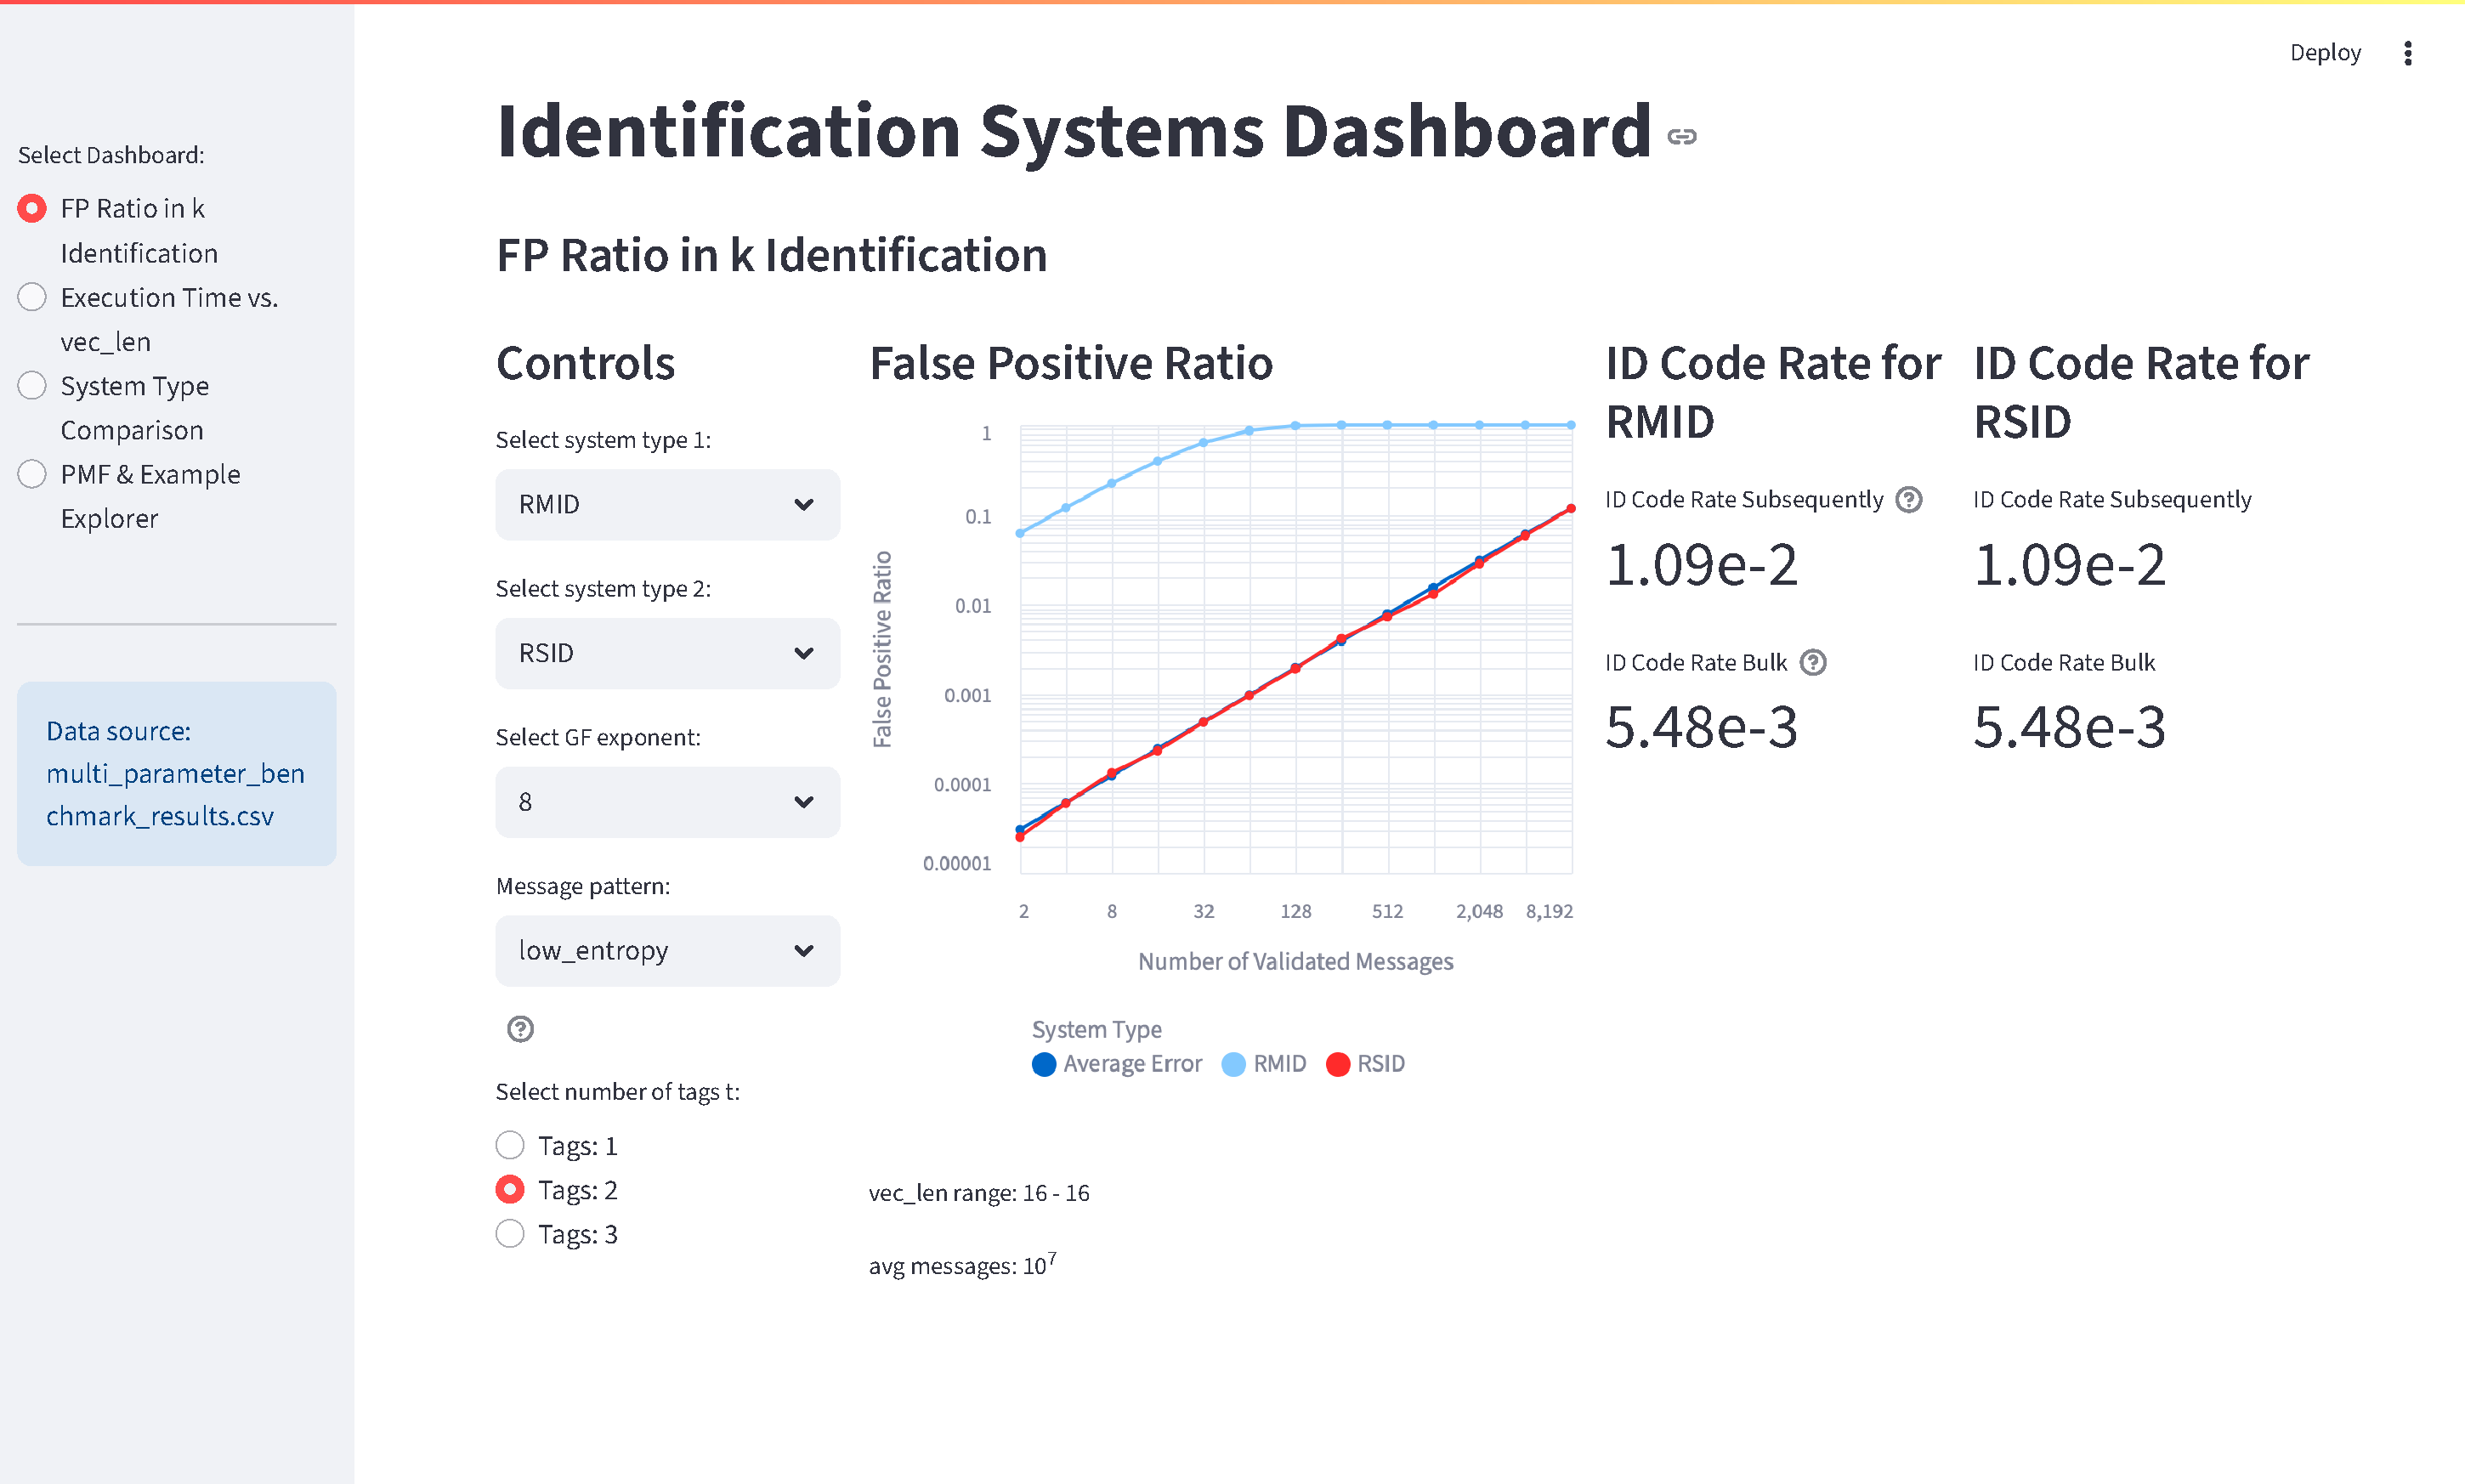
\includegraphics[width=\textwidth]{images/k-identification_dash.pdf}
  \caption{Dashboard panel for k-Identification analyses.}
  \label{fig:dashKID}
\end{figure}

\begin{figure}[hp]
  \centering
  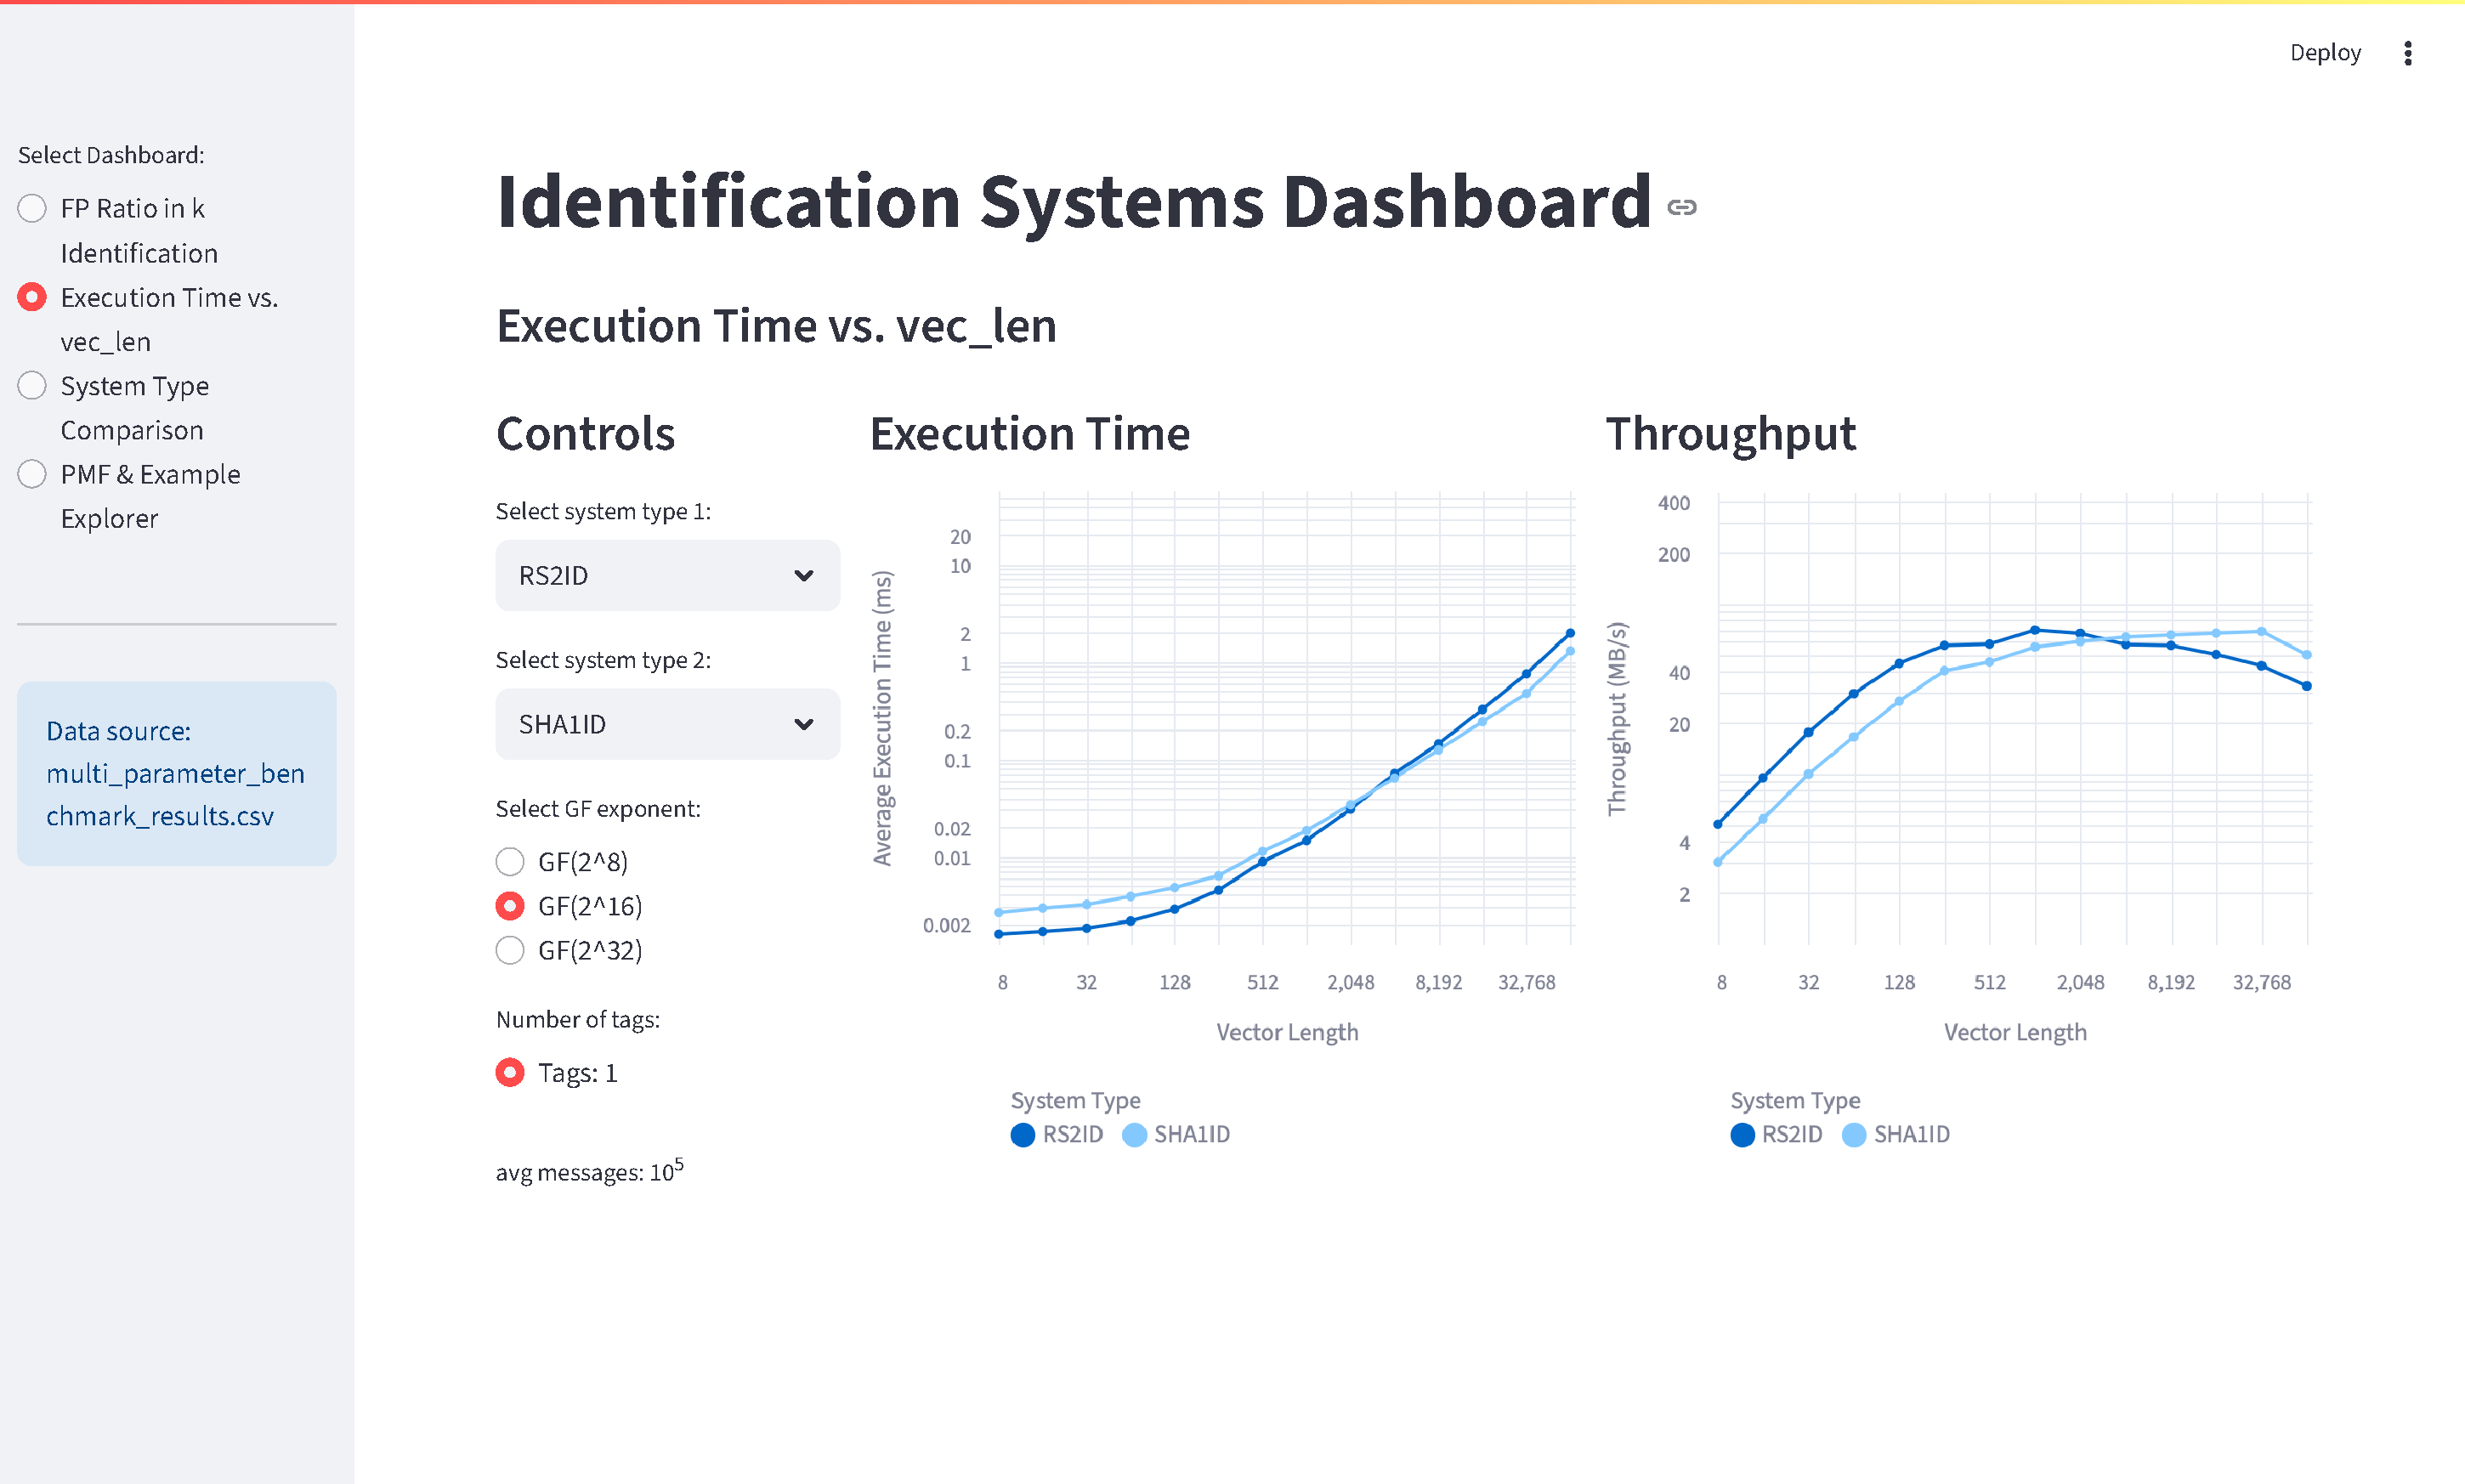
\includegraphics[width=\textwidth]{images/execution_time_dash.pdf}
  \caption{Dashboard panel for execution time analyses.}
  \label{fig:dashExecTime}
\end{figure}

\begin{figure}[hp]
  \centering
  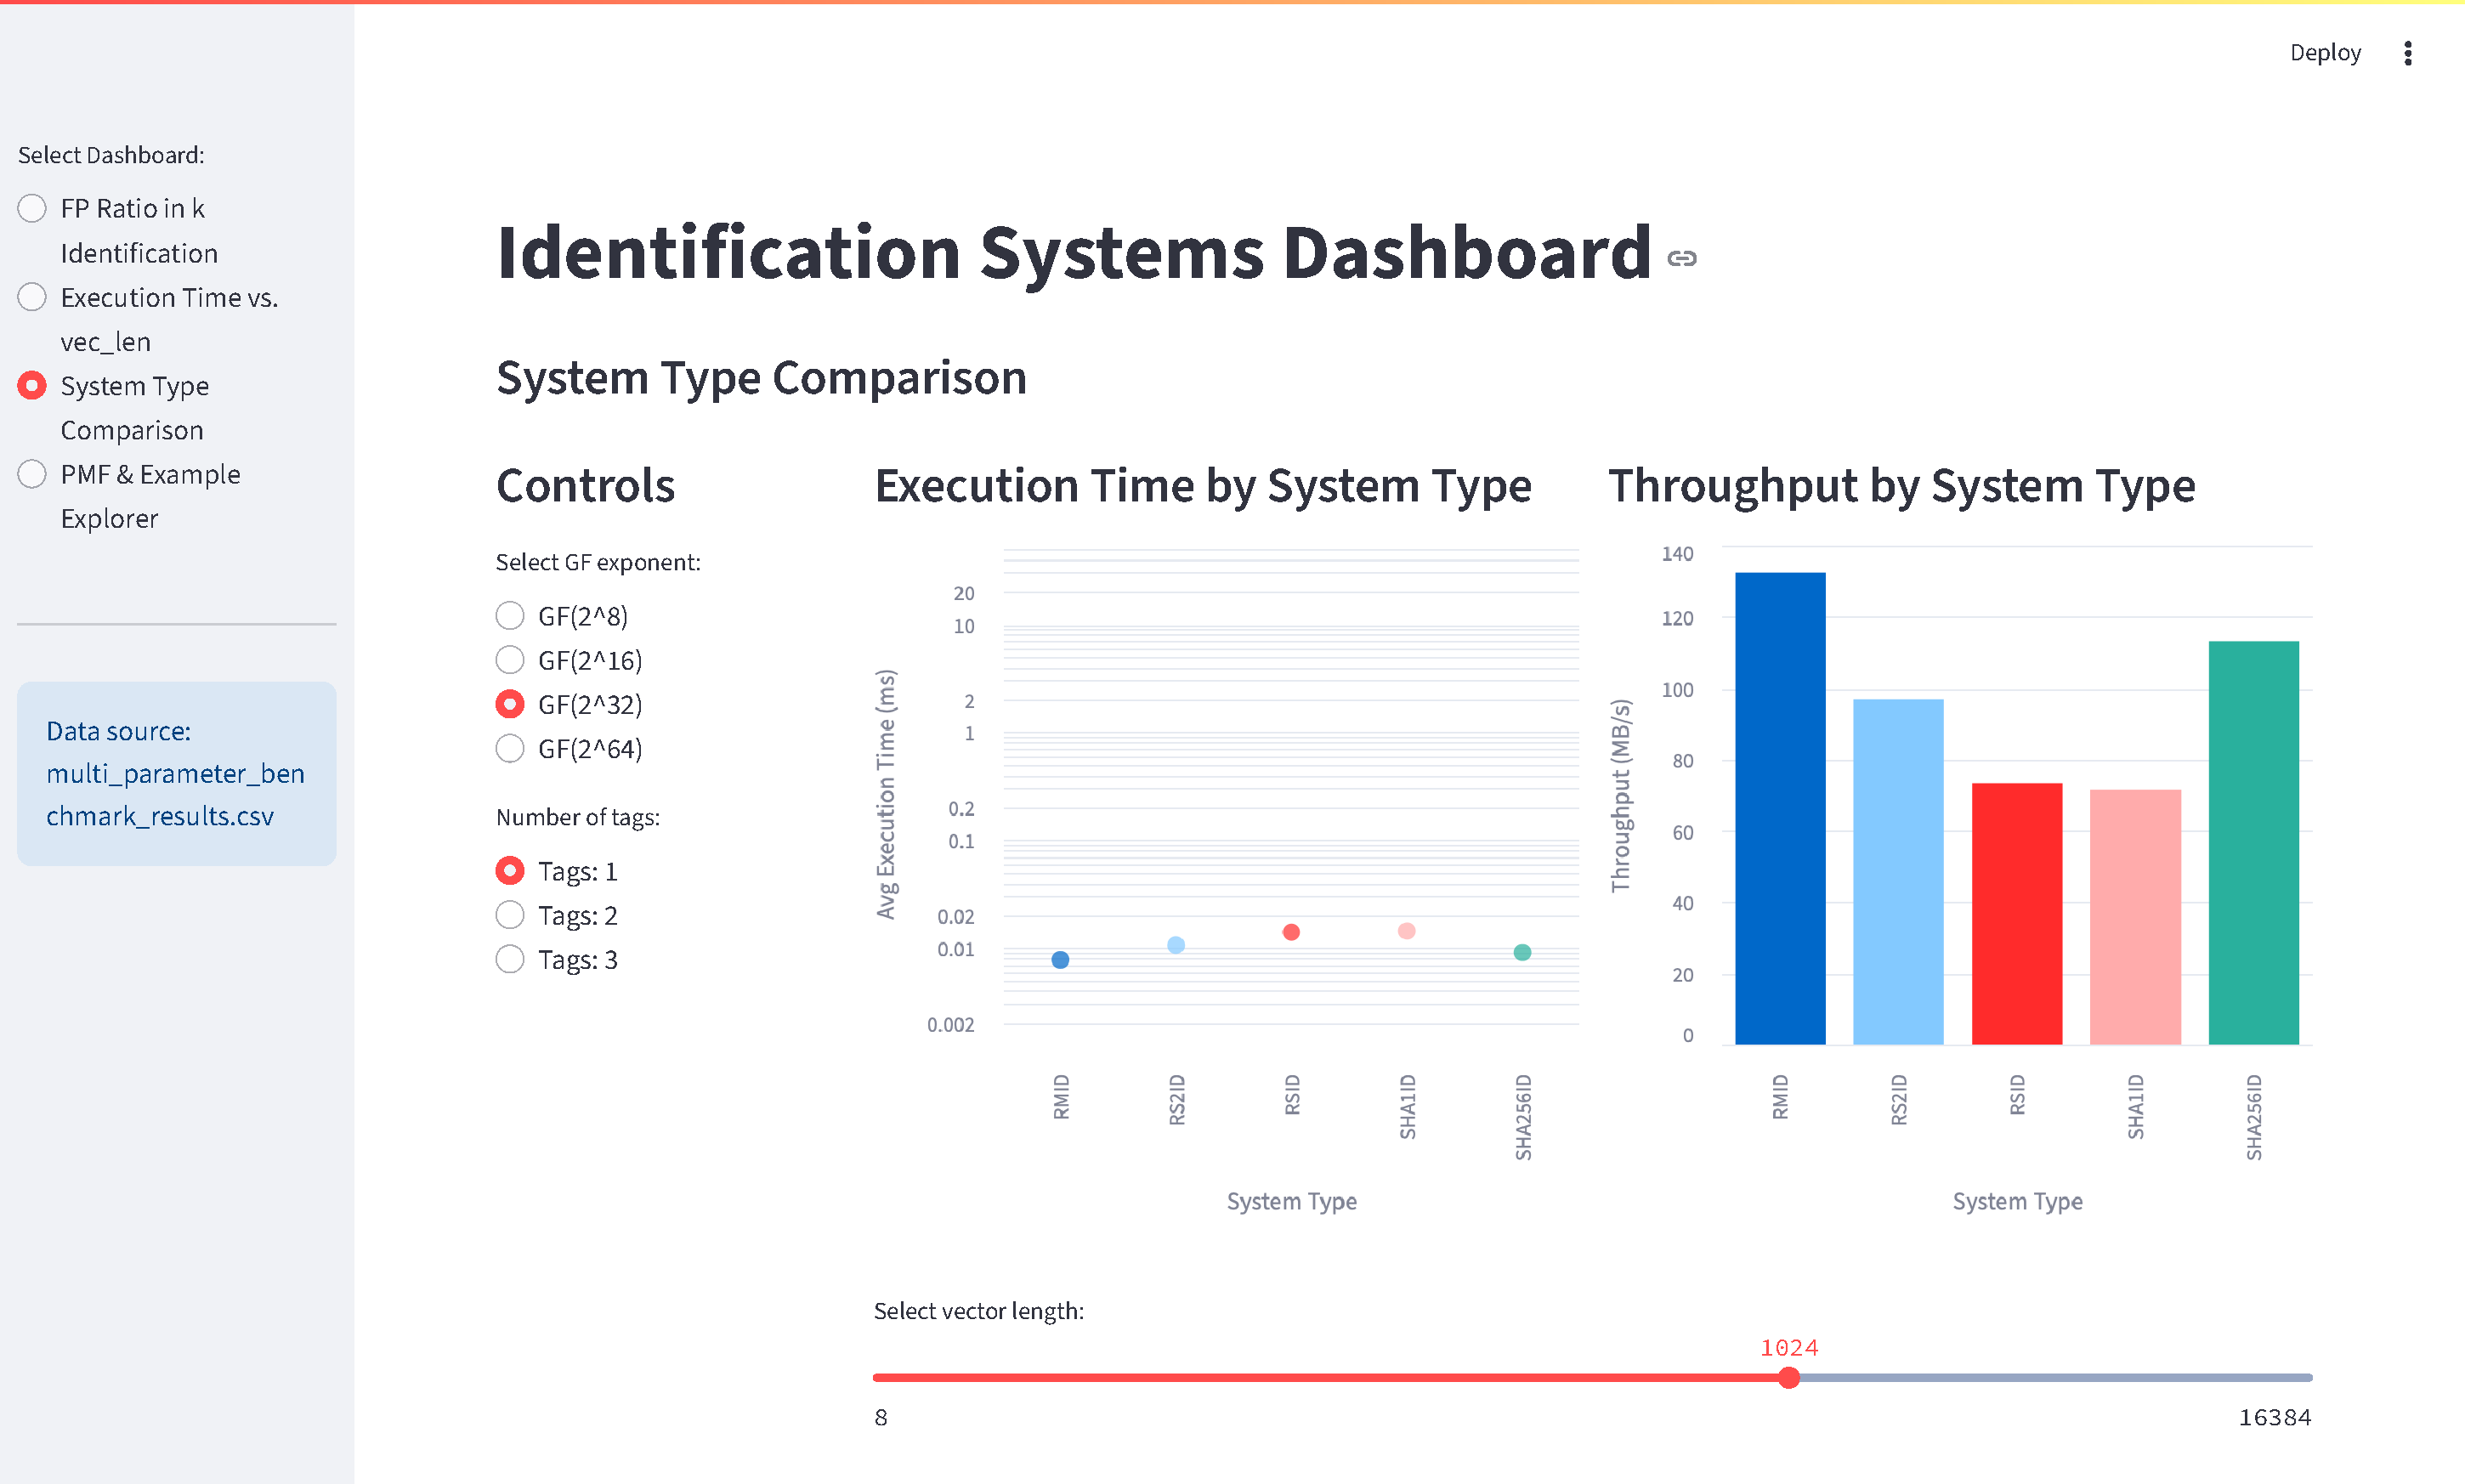
\includegraphics[width=\textwidth]{images/system_comparison_dash.pdf}
  \caption{Dashboard panel for system comparison.}
  \label{fig:dashSysComp}
\end{figure}

\begin{figure}[hp]
  \centering
  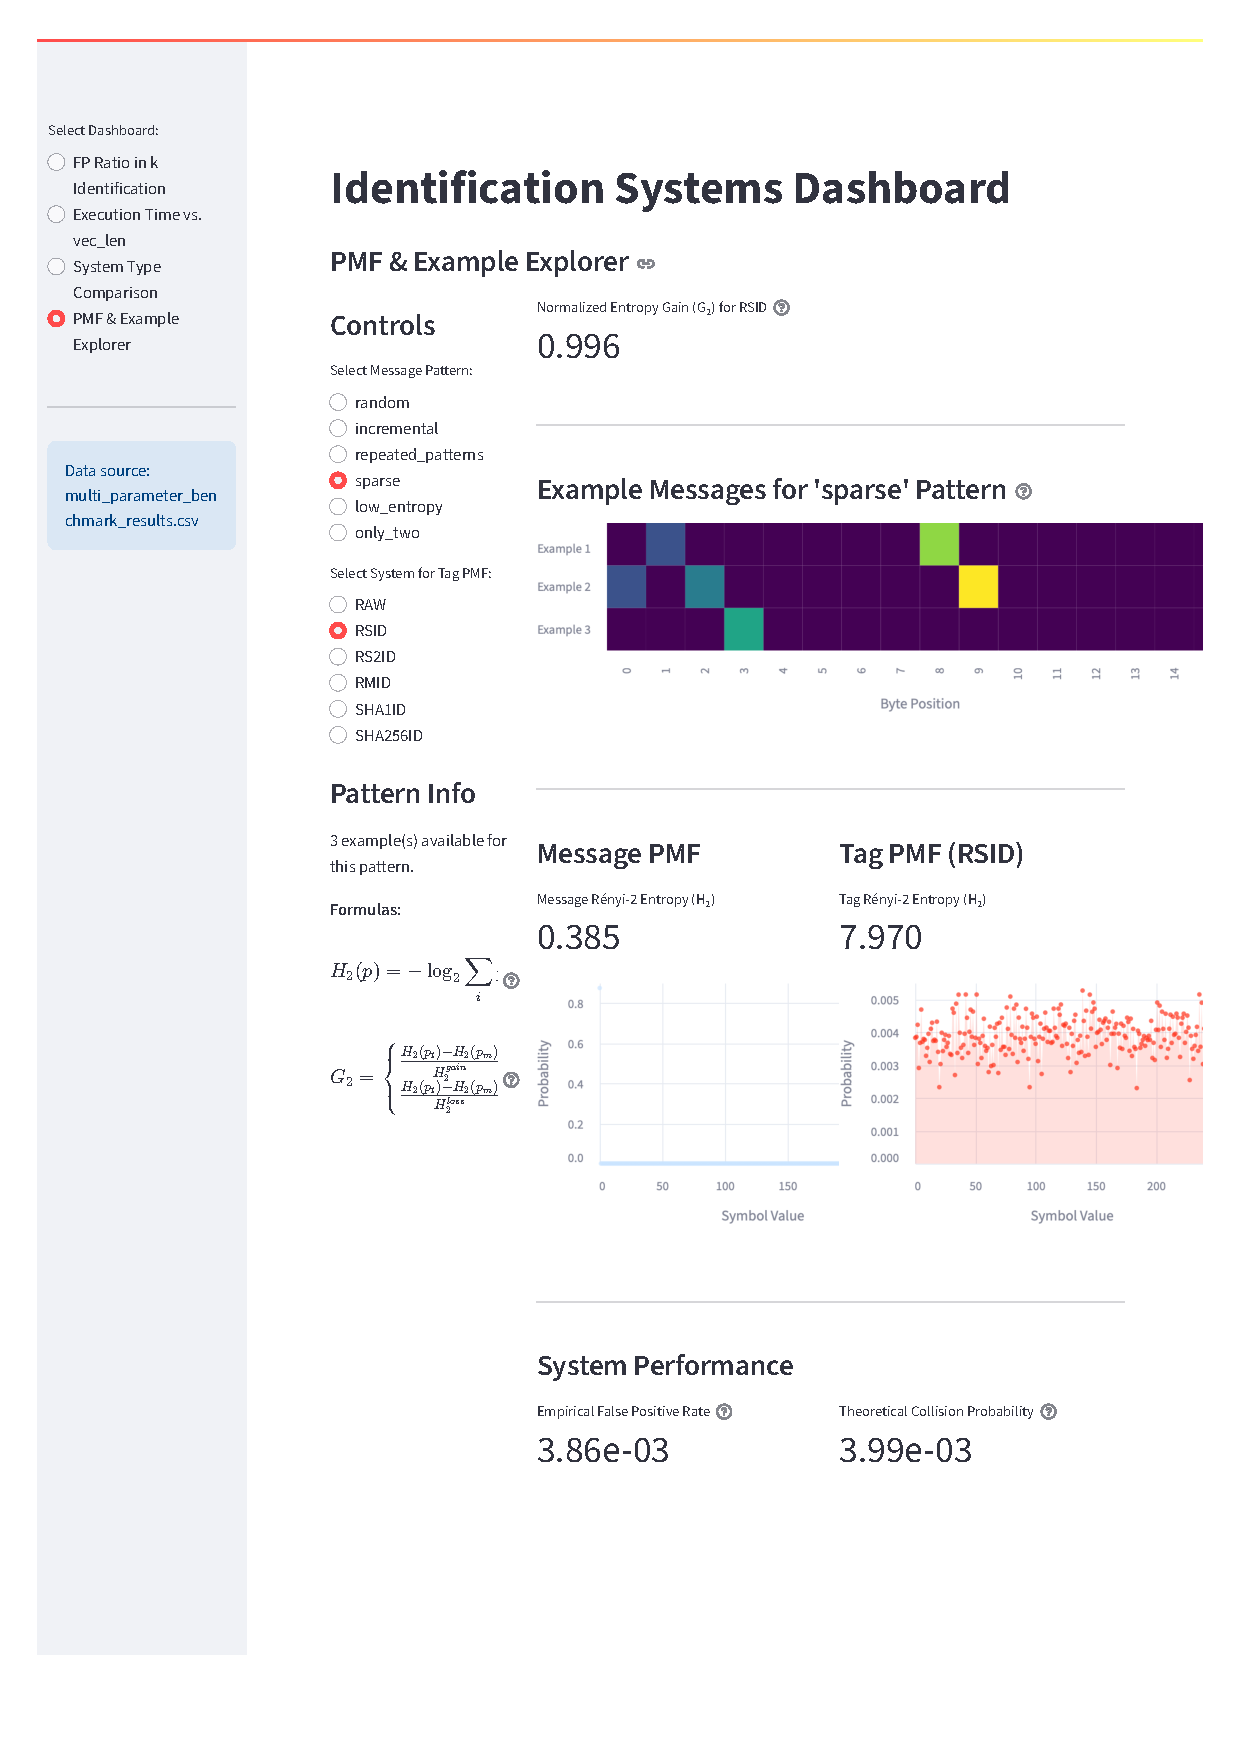
\includegraphics[width=\textwidth]{images/pmf_dash.pdf}
  \caption{Dashboard panel for PMF analysis.}
  \label{fig:dashPMF}
\end{figure}

\end{document}